\documentclass[aspectratio=169,xcolor=dvipsnames]{beamer}
\usetheme{SimplePlus}

% Math
\usepackage{nicefrac}

% Tipography stuff
\usepackage{booktabs} % Allows the use of \toprule, \midrule and \bottomrule in tables
\usepackage[english]{babel}
\usepackage{csquotes}
\usepackage{microtype}
\usepackage{pdfpages}
\usepackage{fontawesome5}
\usepackage{soul}
\usepackage{euler}
\usepackage{algorithm2e}
\usepackage{animate}
\usepackage{ifthen}
\usepackage{multirow}

% Bibliography
\usepackage[giveninits,style=authoryear-comp,backend=biber]{biblatex}
\addbibresource{../fracbiblio.bib}
\newcommand\unnumbered{\setbeamertemplate{footline}{}}%\addtocounter{framenumber}{-1}
\renewcommand*{\bibfont}{\normalfont\small}

% Figures
\usepackage{tikz,pgfplots}
\usetikzlibrary{calc,arrows,patterns,matrix,external}
\usepackage{subfig}
\usepackage{graphicx} % Allows including images
\usepackage[american]{circuitikz}
\usepackage{tikz-network}
\tikzexternalize[prefix=Figures/] % activate and define figures/ as cache folder
\usepackage{mathtools}

% Links
\usepackage{hyperref}
\hypersetup{colorlinks,linkcolor=,urlcolor=MidnightBlue}

% Code
\usepackage{minted}

% Block matrices
\newcommand{\bigzero}{\mbox{\normalfont\Large\bfseries 0}}
\newcommand{\rvline}{\hspace*{-\arraycolsep}\vline\hspace*{-\arraycolsep}}
\newcommand{\R}{\mathbb{R}}
\newcommand{\bone}{{\bf 1}}
\newcommand{\evec}{{\bf e}}
\newcommand{\dvec}{{\bf d}}
\newcommand{\xvec}{{\bf x}}
\newcommand{\yvec}{{\bf y}}
\newcommand{\qvec}{{\bf q}}
\newcommand{\svec}{{\bf s}}
\newcommand{\pvec}{{\bf p}}
\newcommand{\tvec}{{\bf t}}
\definecolor{Ao}{rgb}{0.0, 0.5, 0.0}
\setlength{\tabcolsep}{0.3em}


\author{Fabio Durastante}
\title{An introduction to fractional calculus}
\subtitle{Fundamental ideas and numerics}
\institute{Università di Pisa\\\href{mailto:fabio.durastante@unipi.it}{\faEnvelope\;fabio.durastante@unipi.it}\\\href{https://fdurastante.github.io}{\faFirefox\;fdurastante.github.io}}
\date{October, 2022}

\newcommand{\de}{{\rm d}}


\begin{document}
	
	{\unnumbered
		\begin{frame}[t,plain,noframenumbering]
			\titlepage
			\vspace{-4em}
\includegraphics[width=2cm]{frame.png}
		\end{frame}
	}

	\section{The curse of dimensionality}
	
	\begin{frame}{\faBookDead\,The curse of dimensionality}
	
	In the last lesson we saw that:
	\begin{itemize}
		\item[\faExclamationCircle]<1-> Circulant preconditioners \textbf{cannot cluster} cases with variable coefficients,
		\item[\faExclamationCircle]<2-> Multilevel circulant preconditioners \textbf{cannot cluster} multilevel Toeplitz systems,
		\item[\faExclamationCircle]<3-> Preconditioner based on matrix algebras with fast simultaneous diagonalization \textbf{cannot cluster} multilevel Toeplitz systems.
		\item[\alert{\faQuestionCircle}]<4-> Can we \alert{\textbf{reduce the dimensionality}} of the problem to reuse the information and good results we have in the 1D case?
		\begin{itemize}
			\item[\faWrench]<5-> \normalsize Alternating-direction implicit method,
			\item[\faWrench]<6-> \normalsize reformulation as \emph{matrix equations},
			\item[\faWrench]<7-> \normalsize reformulation as \emph{tensor problems}.
		\end{itemize}
	\end{itemize}
	
	\end{frame}

	\subsection{Matrix equation reformulations}

	\begin{frame}{Matrix equation reformulations}
	
	The simplest way of introducing this reformulation is to go back to the 1D problem (now with a \emph{source term}):
	\begin{equation*}
		\begin{cases}\frac{\partial W}{\partial t} = \theta\,{}^{\only<1>{RL}\only<2->{\alert<2>{GL}}}D_{[0,x]}^\alpha W(x,t) + (1-\theta) {}^{\only<1>{RL}\only<2->{\alert<2>{GL}}}D_{[x,1]}^\alpha W(x,t) + f(x,t), \qquad \theta \in [0,1],\\
			W(0,t) = W(1,t) = 0, \qquad W(x,t) = W_0(x).	
		\end{cases}
	\end{equation*}
	\onslide<2->{To solve everything we have to solve the \textbf{sequence of linear systems}
	\[
	\frac{1}{\Delta t} \left( \mathbf{W}^{(m+1)} - \mathbf{W}^{(m)} \right) = \frac{1}{h^\alpha} \left( \theta G_N + (1-\theta) G_N^T \right) \mathbf{W}^{(m+1))} + \mathbf{f}^{(m+1)}, \; m = 0,\ldots,M-1.
	\]
	}
	\onslide<3->{
	\centering \textcolor{Goldenrod}{\faLightbulb}\;Do we really have to solve this sequentially?
	}
	
	\end{frame}

	\begin{frame}{Matrix equation reformulations}
	Following \parencite{MR3498143}, we can \alert{\textbf{collect the time steps altogether}}:
	\[
	\left( B_M \otimes I_N - \frac{\Delta t}{h^\alpha} I_M \otimes T_N \right) \hat{\mathbf{W}} = \mathbf{F},
	\]
	since
	\[
	\begin{bmatrix}
	I_N -  \frac{\Delta t}{h^\alpha} T_N & \\
	-I_N & I_N -  \frac{\Delta t}{h^\alpha} T_N \\
	& \ddots & \ddots \\
	&  -I_N & I_N -  \frac{\Delta t}{h^\alpha} T_N \\
	\end{bmatrix} \begin{bmatrix}
	\mathbf{W}^{(1)} \\
	\mathbf{W}^{(2)} \\
	\vdots \\
	\mathbf{W}^{(M-1)} \\
\end{bmatrix} = \begin{bmatrix}
\textbf{W}^{(0)} + \Delta t\mathbf{f}^{(1)} \\
\Delta t \mathbf{f}^{(2)} \\
\vdots \\
\Delta t \mathbf{f}^{(M)},
\end{bmatrix}
	\]
for $T_N = \left( \theta G_N + (1-\theta) G_N^T \right)$, $B_M = T_M(1-e^{i\theta})$.
\vfill

\onslide<2>{This is now a \textbf{coupled system} of size $MN \times MN$, that is larger and uglier than before$\ldots$}
	
	\end{frame}

	\begin{frame}{Matrix equation reformulations}
	\faQuestionCircle\;Where is the advantage in dealing with
	\[
	\left( B_M \otimes I_N \only<1>{- \frac{\Delta t}{h^\alpha} I_M \otimes T_N}\only<2->{+ I_M \otimes A_N} \right) \hat{\mathbf{W}} = \mathbf{F}\only<2->{,\qquad A_N =  - \frac{\Delta t}{h^\alpha} T_N}?
	\]
	\onslide<3->{
	Let's call $W = [\mathbf{W}^{(1)}|\cdots|\mathbf{W}^{(M)}]_{N \times M}$, $F = [ \mathbf{W}^{(0)} + \Delta t \mathbf{f}^{(1)}|\cdots| \Delta t \mathbf{f}^{M} ]_{N \times M}$, and rewrite our problem as
	\[
	\text{\faHammer\,Compute }W \in \mathbb{R}^{N \times M} \text{ s.t. } A_N W + W B_M^T = F.
	\]
	}
	\begin{itemize}
		\item[\faLightbulb]<4-> This is a well-know object called \alert{\textbf{Sylvester equation}}!
		\item[\faQuestionCircle]<5-> Did we gain anything? \onslide<6->{ Back to this in a few moment$\ldots$}
		\item[\faQuestionCircle]<7-> Since we are accumulating all the time steps in one step, is it appropriate to simply use one of the methods we already know (e.g. Euler, BDFs, Adams', etc.) or can we do better? \onslide<7->{\definecolor{todo}{HTML}{0099cc} \textcolor{todo}{\faClipboardList}\;Next lecture! }
	\end{itemize}
	\end{frame}

	\begin{frame}{What about the 2D problem?}
	What happens if we want then to reformulate:
	\begin{equation*}
		\begin{cases}\frac{\partial W}{\partial t} = \left(\theta\,{}^{\only<1>{RL}\only<2->{\alert<2>{GL}}}D_{[0,x]}^\alpha \cdot + (1-\theta) {}^{\only<1>{RL}\only<2->{\alert<2>{GL}}}D_{[x,1]}^\alpha \cdot \right) W(x,y,t) \\
			 \phantom{\frac{\partial W}{\partial t} =}+\left(\theta\,{}^{\only<1>{RL}\only<2->{\alert<2>{GL}}}D_{[0,y]}^\alpha \cdot + (1-\theta) {}^{\only<1>{RL}\only<2->{\alert<2>{GL}}}D_{[y,1]}^\alpha \cdot \right) W(x,y,t) + f(x,y,t), \qquad \theta \in [0,1],\\
			W(0,t) = W(1,t) = 0, \qquad W(x,t) = W_0(x).	
		\end{cases}
	\end{equation*}
	\onslide<3->{By the usual procedure
	\only<3>{\[\hspace{-2em}
	\begin{split}
	\frac{1}{\Delta t} \left( \mathbf{W}^{(m+1)} - \mathbf{W}^{(m)} \right) = & \frac{1}{h^\alpha}\left( ( \theta G_{N_x} + (1-\theta) G_{N_x}^T ) \otimes I_{N_y} + I_{N_x} \otimes ( \theta G_{N_y} + (1-\theta) G_{N_y}^T ) \right)\mathbf{W}^{(m+1)} \\ & + \mathbf{f}^{(m+1)}, \quad m=0,\ldots,M-1.
	\end{split}
	\]}\only<4>{
	\[
	\begin{split}
	\frac{1}{\Delta t} \left( \mathbf{W}^{(m+1)} - \mathbf{W}^{(m)} \right) = & \left( \tilde{G}_{N_x} \otimes I_{N_y} + I_{N_x} \otimes \tilde{G}_{N_y} \right)\mathbf{W}^{(m+1)} + \mathbf{f}^{(m+1)}, \quad m=0,\ldots,M-1.
	\end{split}
	\]
	}\only<5>{
	\[
	\begin{split}
		\frac{1}{\Delta t} \left( \mathbf{W}^{(m+1)} - \mathbf{W}^{(m)} \right) = & \underbrace{\left( \tilde{G}_{N_x} \otimes I_{N_y} + I_{N_x} \otimes \tilde{G}_{N_y} \right)}_{G_{N_x N_y}}\mathbf{W}^{(m+1)} + \mathbf{f}^{(m+1)}, \quad m=0,\ldots,M-1.
	\end{split}
	\]
	}\only<6-7>{
	\[
	\left(I_{N_x N_y} - \Delta t G_{N_xN_y} \right) \mathbf{W}^{(m+1)} = \mathbf{W}^{(m)} + \Delta \mathbf{f}^{m+1}, \quad m=0,\ldots,M-1.
	\]
	}\only<8->{\[\hspace{-1.5em}
	\left( \frac{1}{2} I_{N_x} - \Delta t \tilde{G}_{N_x} \right) \tilde{W}^{(m+1)} + \tilde{W}^{(m+1)} \left( \frac{1}{2} I^{N_y} - \Delta t \tilde{G}_{N_y} \right)^T = \tilde{W}^{(m)} + \Delta t F^{(m+1)}, \quad m=0,\ldots,M-1.
	\]
	}
	}
	\only<7-8>{
	\faCog\;The \textbf{clever observation} is now that
	\[
	I_{N_x N_y} - \Delta t G_{N_xN_y} = I_{N_y} \otimes \left( \frac{1}{2} I_{N_x} - \Delta t \tilde{G}_{N_x}  \right) + \left( \frac{1}{2} I_{N_y} - \Delta t \tilde{G}_{N_y} \right) \otimes I_{N_x}.
	\]
	}\only<9>{
	\begin{itemize}
	\item[\faWrench] We now have a \alert{\textbf{sequence of Sylvester equations}} for $m = 0,\ldots,M-1$.
	\item[\faExclamationCircle] The matrix coefficients are related to \emph{rescaled} 1D problems.
	\end{itemize}
	}
	\end{frame}

	\subsection{Solving Sylvester equations}
	
	\begin{frame}{Solving Sylvester equations~\parencite{MR3532794}}
	\faMoneyBill\;This rewriting effort will be worth it only if we can \textbf{efficiently solve} Sylvester equations:
	\[
	A X + X B = C, \quad A \in \mathbb{R}^{N \times N}, \; B \in \mathbb{R}^{M \times M}, \quad C \in \mathbb{R}^{N \times M}.
	\]
	\onslide<2->{
	The solution can be expressed in \textbf{closed form} in a number of ways, e.g., \only<2>{
	as \emph{integrals of resolvents}
	\[
	X = - \frac{1}{4\pi^2} \int_{\Gamma_1} \int_{\Gamma_2} \frac{(\gamma I_N - A)^{-1} C (\mu I_M - B)^{-1}}{\lambda + \mu}\,\mathrm{d}\mu\mathrm{d}\lambda,
	\]
	for $\Gamma_1$, $\Gamma_2$ contours containing and sufficiently close to the spectra of $A$ and $B$, respectively.
	}\only<3>{
	as \emph{integrals of exponentials}
	\[
	X = - \int_{0}^{+\infty} e^{A t} C e^{B t}\,\mathrm{d}t,
	\]
	for $A$ and $B$ with a spectra separated by a vertical line.
	}\only<4->{ in the \emph{diagonalizable case}, by means of \emph{similarity transformations}
	\[
	U^{-1} A U = \operatorname{diag}(\lambda_1,\ldots,\lambda_N), \qquad V^{-1}BV = \operatorname{diag}(\mu_1,\ldots,\mu_M), 
	\]
	then
	\[
	X = U \tilde{X} V, \quad \tilde{x}_{i,j} = \frac{1}{\lambda_i + \mu_j} (U^{-1}CV)_{i,j}.
	\]
	}
	}
	\begin{block}<5->{Numerical mehtods}
	These formulations can exploited to devise numerical methods, to avoid a very long detour, we are going to just mention a couple of them; read~\parencite{MR3532794} for the full story.
	\end{block}
	\end{frame}

	\subsubsection{The Bartels and Stewart algorithm}

	\begin{frame}{The \cite{10.1145/361573.361582} algorithm}
	
	\begin{columns}
	\begin{column}{0.5\columnwidth}
	\begin{itemize}
		\item[\faMoneyBillWave]<2-> The first step costs $O(N^3)$ and $O(M^3)$ operations by \textbf{QR algorithm} for general $A$ and $B$,
		\item[\faMoneyBillWave]<3-> The last step is just two matrix-matrix multiplications.
	\end{itemize}
	\end{column}
	\begin{column}{0.45\columnwidth}
	\begin{algorithm}[H]
	\KwIn{$A$, $B$, $C$}
	\alert<2>{Compute Schur factorizations $U R U^H  = A^H$ and $B = V S V^H$}\;
	\alert<4-11>{Solve $R^H Y + Y S = U^H C V$ for $Y$}\;
	\alert<3>{Compute $X = U Y V^H$}\; 
	\end{algorithm}
	\end{column}
	\end{columns}
	\vfill
	
	\onslide<4->{
	We can solve the system with triangular coefficients by substitution
	\only<4>{ 
	\[
	R^H Y + Y S = U^H C V
	\]  }
	\only<5->{
	\[
	\begin{bmatrix}
	\alert<6,7,8>{\spadesuit}  &    &  \\
	\spadesuit & \spadesuit  &  \\
	\spadesuit  & \spadesuit  & \spadesuit \\
 	\end{bmatrix} \begin{bmatrix}
	\only<5-6>{\alert<6>{\times}}\only<7->{y_{1,1}} & \only<5-7>{\alert<7>{\times}}\only<8->{y_{12}} & \only<5-8>{\alert<8>{\times}}\only<9->{y_{1,3}} \\
 	\only<5-10>{\alert<10>{\times}}\only<11->{y_{2,1}} & \only<5-10>{\alert<10>{\times}}\only<11->{y_{2,2}} & \only<5-10>{\alert<10>{\times}}\only<11->{y_{2,3}} \\
 	\only<5-11>{\alert<11>{\times}}\only<12->{y_{3,1}} & \only<5-11>{\alert<11>{\times}}\only<12->{y_{3,2}} & \only<5-11>{\alert<11>{\times}}\only<12->{y_{3,3}} \\
 	\end{bmatrix} + \begin{bmatrix}
 	\only<5,6>{\alert<6>{\times}}\only<7->{\alert<7,8>{y_{11}}} & \only<5-7>{\alert<7>{\times}}\only<8->{\alert<8>{y_{12}}} & \only<5-8>{\alert<8>{\times}}\only<9->{y_{1,3}}  \\
 	\only<5-10>{\alert<10>{\times}}\only<11->{y_{2,1}} & \only<5-10>{\alert<10>{\times}}\only<11->{y_{2,2}} & \only<5-10>{\alert<10>{\times}}\only<11->{y_{2,3}} \\
 	\only<5-11>{\alert<11>{\times}}\only<12->{y_{3,1}} & \only<5-11>{\alert<11>{\times}}\only<12->{y_{3,2}} & \only<5-11>{\alert<11>{\times}}\only<12->{y_{3,3}} \\
 \end{bmatrix} 	\begin{bmatrix}
 \alert<6>{\clubsuit}  & \alert<7>{\clubsuit}   &  \alert<8>{\clubsuit} \\
  & \alert<7>{\clubsuit}  & \alert<8>{\clubsuit}  \\
   &   & \alert<8>{\clubsuit} \\
\end{bmatrix} = \begin{bmatrix}
\alert<6>{\bigstar} & \alert<7>{\bigstar} & \alert<8>{\bigstar} \\
\bigstar & \bigstar & \bigstar \\
\bigstar & \bigstar & \bigstar \\
\end{bmatrix}
	\]
	}
	\only<6>{$(Y)_{1,1}$ element is readily obtained by solving: $ (\spadesuit + \clubsuit) (Y)_{11} = \bigstar$.}
	\only<7->{Then we proceed with the first row$\ldots$}\only<9->{ and every other row.}
	}

	\onslide<12->{$\Rightarrow$\;The \alert{\textbf{leading cost}} is the Schur factorization $O(N^3 + M^3)$!\,\alert{\faSadTear}\, only \textbf{small matrices}. }
	
	\onslide<13->{\textcolor{Goldenrod}{\faLightbulb}\;We may gain something if $A$ and $B$ are in \textbf{upper Hessenberg form}$\ldots$}
	\end{frame}

	\begin{frame}{The small case scenario}
	
	There are a number of variations that we can apply for the case of small matrices 
	
	\begin{itemize}
		\item[\faWrench]<2-> We can use \textbf{real Schur form} instead of the complex one, avoids complex arithmetic, but now for in the second step we have to solve some Sylvester equation with $2 \times 2$ coefficients. We do it by going back to a small linear system.
		\item[\faWrench]<3-> We can go directly for the Hessenberg form instead of Schur~\parencite{1102170}.
		\item[\faWrench]<4-> If $A$ is much larger than $B$ then we can work on the block case\onslide<6->{.}
		\only<4-5>{\[
		\begin{bmatrix}
		A_{11} & A_{12} \\
		& \alert<5>{A_{22}}
		\end{bmatrix} \begin{bmatrix} 
		X_1 \\
		\alert<5>{X_2} 
	\end{bmatrix} + \begin{bmatrix}
	X_1 \\
	\alert<5>{X_2} 
\end{bmatrix} \alert<5>{B} = \begin{bmatrix}
C_1 \\
\alert<5>{C_2}
\end{bmatrix}.
		\]}
		\item[\faWrench]<6-> If $B = -A$ and $C$ is \emph{small rank}, then we are falling back to our ``fast small-displacement-rank solver'' scenario, e.g., \parencite{MR1312096}.
	\end{itemize}
	\only<6->{
	\begin{block}<7->{\only<7>{\faSadCry}\only<8>{\faSmileWink}\;But our cases are not small$\ldots$}
	If only we knew a way to from a large matrix setting, to a small one made of Hessenberg matrices$\ldots$\only<8>{ wait a second, we may know a trick or two for this!\;\faSmileWink[regular]}
	\end{block}
	}
	
	\end{frame}

	\subsubsection{Projection methods}
	
	\begin{frame}{When in doubt: project!}
	When we have to solve \textbf{linear systems} with a \textbf{large matrix}, we have seen that a good solution is represented by the \alert{Krylov projection methods}.\vfill 
	
	\faQuestionCircle\; Can we do something similar for this problem too? \onslide<2>{\emph{sometimes}, it is a \textbf{matter of rank}.}
	
	\begin{alertblock}{Theorem~\parencite[Theorem~4]{MR3532794}}
	Let $A$ and $B$ be stable\textsuperscript{1} and real symmetric, with spectra contained in $[a,b]$ and $[c,d]$, respectively. Define $\eta = 2(b-a)(d-c)/((a+c)(b+d))$. Assume $C$ is of \textbf{rank} $p$. Then the singular values $\sigma_1 \geq \cdots \geq \sigma_{\min\{M,N\}}$ of the solution $X$ to the Sylvester equation satisfy
	\[
	\frac{\sigma_{pr+1}}{\sigma_1} \leq \left( \frac{1 - \sqrt{k'_r}}{1+\sqrt{k'_r}} \right)^2, \; 1 \leq pr < n, \; k'_r = \frac{1}{1+\eta+\sqrt{\eta(\eta+2)}}.
	\]
	\end{alertblock}
	
	\footnotetext[1]{A matrix is called stable (or sometimes \emph{Hurwitz}) if every eigenvalue has strictly negative real part.}
	
	\end{frame}

	\begin{frame}{Projection methods for low-rank right-hand sides}
	Let us \textbf{assume} that $\operatorname{rank}{(C)} = p \ll \min\{n,m\}$.
	\begin{itemize}
		\item[\faCog]<2-> Decompose $C = C_1 C_2^H$;
		\item[\faCog]<3-> Select $\mathcal{V} = \operatorname{span}(V_k)$ and $\mathcal{W} = \operatorname{span}(W_j)$ subspaces of $\mathbb{C}^{N}$ and $\mathbb{C}^M$;
		\item[\faCog]<4-> Basis $V_k$, $k \ll N$, and $W_j$, $j \ll M$,  are \emph{orthonormal} and such that $\mathcal{V}$ and $\mathcal{W}$ are not orthogonal to $\operatorname{range}(C_1)$ and $\operatorname{range}(C_2)$ respectively;
		\item[\faCog]<5-> Build an approximation $\tilde{X} = V_k Y W_j^H \approx X$ with residual $R = C_1C_2^H - A \tilde{X} - \tilde{X}B$.
	\end{itemize}
	\begin{exampleblock}<6->{Galerkin (orthogonality) condition}
	Call $\tilde{\mathbf{x}} = \operatorname{vec}(\tilde{X}) = (W_j \otimes V_k)\operatorname{vec}(Y)$, then we want $V_k$ and $W_k$ to be selected as
	\[
	(W_j \otimes V_k)^H (\mathbf{c} - \mathcal{A} \mathbf{x}) = 0 \,\Leftrightarrow \, V_k^H R W_j = 0 \text{ with } \mathcal{A} = B^T \otimes I + I \otimes A, \, \mathbf{c} = \operatorname{vec}(C).
	\]
	\end{exampleblock}
	\begin{itemize}
		\item[\faWrench]<7-> To compute $Y$, solve the \textbf{small Sylvester equation}:
		\[
		V_k^H A V_k Y + Y W_j^H B W_j = V_k^H C_1 (W_j^H C_2)^H\only<7>{.}\onslide<8->{ \alert{\Rightarrow} \text{Bartels and Stewart}.}
		\]
	\end{itemize}
	\end{frame}

	\begin{frame}{Projection methods for low-rank right-hand sides}
	\begin{onlyenv}<1>\begin{block}{Existence of the solution}
	If $V_k^H A V_k$ and $- W_j^H B W_j$ have \textbf{disjoint spectra} we can solve 
	\[
	V_k^H A V_k Y + Y W_j^H B W_j = V_k^H C_1 (W_j^H C_2)^H \qquad \forall\,C = C_1 C_2^H.
	\]
	To enforce it, is sufficient to have $A$ and $-B$ with disjoint field of values.
	\end{block}\end{onlyenv}\begin{onlyenv}<2->
	\begin{columns}
	\begin{column}{0.4\columnwidth}
	The cost of \textbf{one iteration} for $m > n$ and $p = \operatorname{rank}(C)$ is then given by
	\begin{itemize}
		\item[\faMoneyBillWave]<3-> $O((kp)^3)$ flops for the solution of the projected problem,
		\item[\faMoneyBillWave]<4-> Orthogonalization of the new basis vectors with respect to the older vectors: $O(mkp^2)$,
		\item[\faMoneyBillWave]<5-> Orthogonalization of the new block: $O(mp^2)$.
	\end{itemize}\vspace{-0.7em}
	\begin{block}<6->{Loss of rank}
	If the generated basis experiences loss of rank, deflation procedures can be applied to remove redundant columns.
	\end{block}
	\end{column}
	\begin{column}{0.6\columnwidth}
	\begin{algorithm}[H]\small
	\KwIn{$A$, $B$, $C_1$ and $C_2$}
	Orthogonalize columns of $C_1$ to get $\mathbf{v}_1 = V_1$\;
	Orthogonalize columns of $C_2$ to get $\mathbf{v}_2 = W_1$\;
	\For{$k=1,2,\ldots,$}{
		\alert<3>{Compute $Y_k$ solution to $V_k^H A V_k Y + Y W_k^H B W_k - V_k^H C_1 (W_k^H C_2)^H = 0$}\;
		\If{\emph{converged}}{
			Return $V_k$, $Y_k$ and $W_k$ such that $X_k = V_k Y_k W_k^*$ and \textbf{stop}.	
		}
	\tcc{Compute next bases blocks}
	\alert<7>{Compute $\tilde{{v}}$ and $\hat{{w}}$ from the \textbf{approximate space}}\;
	\alert<4>{Make $\hat{{v}}$ orthogonal w.r.t. $\{\mathbf{v}_1,\ldots,\mathbf{v}_k\}$}\;
	\alert<4>{Make $\hat{{w}}$ orthogonal w.r.t. $\{\mathbf{w}_1,\ldots,\mathbf{w}_k\}$}\;
	\alert<5>{Orthogonalize col.s of $\hat{\mathbf{v}}$ and $\hat{\mathbf{w}}$ for $\mathbf{v}_{k+1}$ and $\mathbf{w}_{k+1}$}\;
	Update: $V_{k+1} = [V_k,\mathbf{v}_{k+1}]$, $W_{k+1} = [W_k,\mathbf{w}_{k+1}]$\;
	}
	\end{algorithm}
	\end{column}
	\end{columns}
	\end{onlyenv}
	\end{frame}

	\begin{frame}{Selection of $\mathcal{V}$ and $\mathcal{W}$}
	\faQuestionCircle\;How do we select the approximation spaces $\mathcal{V}$ and $\mathcal{W}$?
	\begin{itemize}
		\item[\faDoorOpen] Standard \textbf{block} Krylov subspace
		\[ \mathcal{V} = \operatorname{range}\{[C_1,AC_1,A^2C_2,\ldots] \}, \quad \mathcal{W} = \operatorname{range}\{[C_2,B^HC_1,(B^H)^2C_2,\ldots] \}, \]
		\item[\faDoorOpen] Rational \textbf{block} Krylov subspace
		\[ 
		\begin{split}
		\mathcal{V} = &\;\operatorname{range}\{[ (A+ \sigma_1 I)^{-1} C_1, (A+ \sigma_2 I)^{-1} (A+ \sigma_1 I)^{-1} C_1,\ldots] \}, \\ \mathcal{W} = &\; \operatorname{range}\{[ (B^H + \eta_1 I)^{-1} C_2, (B^H+ \eta_2 I)^{-1} (B^H+ \eta_1 I)^{-1} C_2,\ldots] \},
		\end{split}
		 \]
		 \item[\faDoorOpen] Global Krylov subspace:
		 \[
		 \mathcal{V} = \left\lbrace \sum_{i \geq 0} A^i C_i \gamma_i, \quad \gamma_i \in \mathbb{R} \right\rbrace = \operatorname{span}\{C_1,AC_1,A^2C_2,\ldots \}
		 \]
		 where the linear combination is performed blockwise, and analogously for $\mathcal{W}$.
	\end{itemize}
	\end{frame}

	\begin{frame}{Stopping criterions}
	To change the ``\textbf{if} \emph{converged}'' in the algorithm we have to monitor the residual, e.g.,
	\[
	\| R \|_2 = \| A \tilde{X} + \tilde{X} B - C_1 C_2^*\|_2 \text{ or } \| R \|_F = \| A \tilde{X} + \tilde{X} B - C_1 C_2^*\|_F.
	\]
	\begin{itemize}
		\item[\alert{\faExclamationTriangle}]<2-> $R$ is \textbf{dense} and \textbf{large}: we should avoid assembling it!
		\item[\faExclamationCircle]<3-> If we are using Krylov subspaces, we can employ Arnoldi-like relations to this end:
		\[
		A V_k = [V_k,\hat{v}_k] \underline{H}_k \text{ and } B^H W_j = [W_j,\hat{w}_j] \underline{K}_j, 
		\]
		with $[V_k,\hat{v}_k]$ and $[W_j,\hat{w}_j]$ having orthonormal columns.
		\item[\faWrench]<3-> If $\exists\, C^{(k)}_1$ and $C^{(j)}_2$ s.t. $C_1 = [V_k,\hat{v}_k]C^{(k)}_1$ and $C_2 = [W_j,\hat{w}_j]C^{(j)}_2$
		\[
		\begin{split}
			\|R\|_F  \only<3>{=& \; \| A V_k Y W_j^H + V_k Y W_j^H B - \hat{V}_k C_1^{(k)} (\hat{W}_j C_2^{(j)})^H \|_F \\
			= & \; \left\|  [V_k \hat{v}_k] \left( \underline{H}_k Y [I,0] + [I;0] Y \underline{K}_j^H - C_1^{(k)} (C_2^{(j)})^H \right) [W_j,\hat{w}_j]^H \right\|_F \\}
			= & \; \|\alert<4>{\underline{H}_k Y [I,0] + [I;0] Y \underline{K}_j^H - C_1^{(k)} (C_2^{(j)})^H }\|_F.
		\end{split}
		\]
		\item[\faMoneyBill]<4-> The matrix in the last norm is small \textbf{if} $k$ and $j$ are small, if we are under the \faWrench\;conditions on the spaces we can \textbf{monitor the residual along the way}.
	\end{itemize}
	\end{frame}

	\begin{frame}{Variants: as many as for standard Krylov methods}
	\begin{itemize}
		\item[\faArrowCircleRight]<1-> We can use different approximation space dimensions for $A$ and $B$.
		\item[\faArrowCircleRight]<2-> We can use different approximation spaces of the same dimension.
		\item[\faArrowCircleRight]<3-> We could use nonsymmetric Lanczos (\emph{oblique} subspaces) if $B = A^H$ and $C_1 C_2^*$ is nonsymmetric to build simultaneously $K_j(A,C_1)$ and $K_j(A,C_2)$.
		\item[\faArrowCircleRight]<4-> We could use Krylov methods with restart to save memory.
		\item[\faArrowCircleRight]<5-> If $A$ and $B$ are symmetric (and not necessarily equal), we could use short-term block recurrences.
	\end{itemize}
	\onslide<6->{\faBook\;The review by \cite{MR3532794} has pointers to all the different strategies available.}
	
	\begin{exampleblock}<7->{\faQuestionCircle[]\;Where were we?}
	For the two equations we wanted to solve we have then the following questions:
	\begin{itemize}
		\item[\faQuestionCircle] Is our $C$ low-rank?
		\item[\faQuestionCircle] What type of Krylov subspace should we select?
		\item[\faQuestionCircle] Does any of this stuff converge at all?
	\end{itemize}
	\end{exampleblock}
	
	\end{frame}

	\subsection{Low-rank, regularity and separability}
	
	\begin{frame}{Low-rank, regularity and separability}
	\faWrench\;For the 1D+1D case we have to solve
	\[
	A_N W + W B_M^T = F, \text{ with } F = [ \mathbf{W}^{(0)} + \Delta t \mathbf{f}^{(1)}|\cdots| \Delta t \mathbf{f}^{M} ]_{N \times M},
	\]
	with $(\mathbf{f}^{(m)})_i = f(x_i,t_m)$.\vfill
	
	\onslide<2->{\faWrench\;For the 1D+2D case we have to solve for $m=0,\ldots,M-1$
	\[
		\left( \frac{1}{2} I_{N_x} - \Delta t \tilde{G}_{N_x} \right) \tilde{W}^{(m+1)} + \tilde{W}^{(m+1)} \left( \frac{1}{2} I^{N_y} - \Delta t \tilde{G}_{N_y} \right)^T = \tilde{W}^{(m)} + \Delta t F^{(m+1)}, \
	\]
	with $(F^{(m+1)})_{i,j} = f(x_i,y_j,t_{m+1})$.}

	\begin{block}<3->{\faQuestionCircle\;Low-Rank}
	When is it that these matrices have a fixed, size-independent ``small'' rank?
	\end{block}
	\end{frame}

	\begin{frame}[fragile]{Low-rank, regularity and separability}
	\faLightbulb\; If a function $f(x,y) = f_1(x)f_2(y)$ then
	\[
	\only<1>{\begin{bmatrix}
	f(x_1,y_1) & f(x_1,y_2) & \cdots & f(x_1,y_n) \\
	f(x_2,y_1) & f(x_2,y_2) & \cdots & f(x_2,y_n) \\
	\vdots & \vdots & \ddots & \vdots \\
	f(x_n,y_1) & f(x_n,y_2) & \cdots & f(x_n,y_n) \\
	\end{bmatrix}}\onslide<2->{	\begin{bmatrix}
	f_1(x_1)f_2(y_1) & f_1(x_1)f_2(y_2) & \cdots & f_1(x_1)f_2(y_n) \\
	f_1(x_2)f_2(y_1) & f_1(x_2)f_2(y_2) & \cdots & f_1(x_2)f_2(y_n) \\
	\vdots & \vdots & \ddots & \vdots \\
	f_1(x_n)f_2(y_1) & f_1(x_n)f_2(y_2) & \cdots & f_1(x_n)f_2(y_n) \\
\end{bmatrix}} \onslide<3->{= \begin{bmatrix}
	f_1(x_1) \\
	f_1(x_2) \\
	\vdots \\
	f_1(x_n) 
	\end{bmatrix} \begin{bmatrix}
	f_2(y_1) & f_2(y_2) & \cdots & f_n(y_n)
\end{bmatrix}}
	\] 
	\begin{onlyenv}<4>
\faEye\; To have a simple example:\vspace{-0.5em}\definecolor{bg}{rgb}{0.95,0.95,0.95}
\begin{minted}[bgcolor=bg,fontsize=\small,breaklines]{matlab}
n = 10;
f1 = @(x) exp(-2*x); f2 = @(y) sin(2*pi*y); f = @(x,y) f1(x).*f2(y);
x = linspace(0,1,n); y = linspace(0,1,n);
[X,Y] = meshgrid(x,y);
A = f(X.',Y.'); a1 = f1(x); a2 = f2(y);
norm(A-a1.'*a2)
\end{minted}
that answers us \mintinline{matlab}{>> ans = 0}.
	\end{onlyenv}
	\begin{onlyenv}<5->
	What happens if $f(x,y)$ is not separable? E.g., if $f(x,y) = \sin(\pi(x+y))$?
	\begin{onlyenv}<5>
	\begin{columns}
	\begin{column}{0.5\columnwidth}\definecolor{bg}{rgb}{0.95,0.95,0.95}
\begin{minted}[bgcolor=bg,fontsize=\small,breaklines]{matlab}
n = 10;
f = @(x,y) sin(pi*(x+y));
x = linspace(0,1,n); 
y = linspace(0,1,n);
[X,Y] = meshgrid(x,y); A = f(X.',Y.'); 
sv = svd(A);
\end{minted}
	\end{column}
	\begin{column}{0.5\columnwidth}
	% This file was created by matlab2tikz.
%
%The latest updates can be retrieved from
%  http://www.mathworks.com/matlabcentral/fileexchange/22022-matlab2tikz-matlab2tikz
%where you can also make suggestions and rate matlab2tikz.
%
\definecolor{mycolor1}{rgb}{0.00000,0.44700,0.74100}%
%
\begin{tikzpicture}

\begin{axis}[%
width=0.7\columnwidth,
height=0.9in,
at={(0.758in,0.481in)},
scale only axis,
xmin=1,
xmax=10,
ymode=log,
ymin=1e-20,
ymax=100000,
yminorticks=true,
axis background/.style={fill=white}
]
\addplot [color=mycolor1, only marks, mark=o, mark options={solid, mycolor1}, forget plot]
  table[row sep=crcr]{%
1	4.9749371855331\\
2	4.9749371855331\\
3	8.42013570898238e-16\\
4	6.78060181120481e-16\\
5	4.37465944793928e-16\\
6	3.68952230751576e-16\\
7	2.3661953224555e-16\\
8	1.11236235206283e-16\\
9	6.38257827716023e-17\\
10	5.68741578311535e-18\\
};
\end{axis}
\end{tikzpicture}%
	\end{column}
	\end{columns}
	\end{onlyenv}
	\begin{onlyenv}<6->
	\[
	\sin(\pi(x+y)) = \sin (\pi  x) \cos (\pi  y)+\cos (\pi  x) \sin (\pi  y)
	\]
	is the \textbf{sum of} two \textbf{separable functions}, i.e., we get a matrix that has rank equal to $2$.
	
	\onslide<7->{\textcolor{Goldenrod}{\faLightbulb}\; We can try to \textbf{generalize} this \textbf{decomposition idea} to more general functions!}
	\end{onlyenv}
	\end{onlyenv}
	\end{frame}

	\begin{frame}[fragile]{Low-rank, regularity and separability}
	We can approximate a function of two variables as the sum of separable functions
	\[
	f(x,y) = \sum_{k=1}^{K} f_k T_k(x)T_k(y), \quad \{T_k(\cdot)\}_{k} \text{ Čebyšëv polynomials.}
	\]
	\vspace{-1em}\begin{exampleblock}{Example (Using \texttt{Chebfun}~\parencite{driscoll2014chebfun})}
	Consider $f(x,y) = \exp( -40(x^2-xy+2y^2 - 1/2)^2)$.
	\end{exampleblock}
\begin{onlyenv}<1>\begin{columns}
\begin{column}{0.6\columnwidth}
\definecolor{bg}{rgb}{0.95,0.95,0.95}
\begin{minted}[bgcolor=bg,fontsize=\small,breaklines]{matlab}
cheb.xy
ff=@(x,y)exp(-40*(x.^2-x.*y+2*y.^2-1/2).^2);
f=chebfun2(ff);
levels = 0.1:0.1:0.9;
contour(f,levels); 
axis([-1 1 -1 1]);
axis square
\end{minted}
\end{column}
\begin{column}{0.4\columnwidth}
\centering

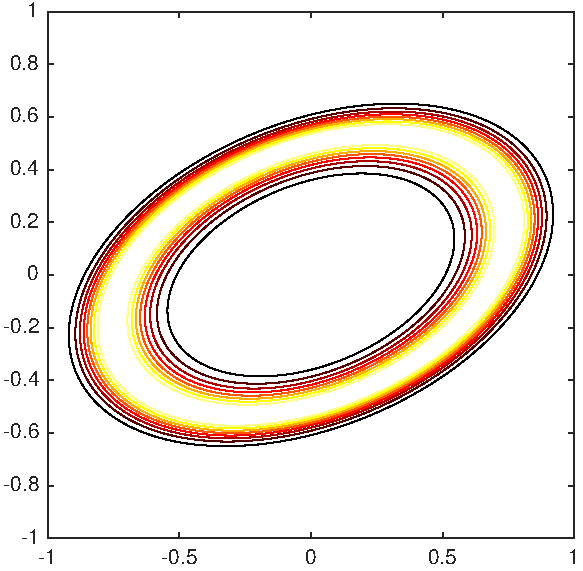
\includegraphics[width=0.7\columnwidth]{chebfun1.pdf}
\end{column}
\end{columns}
\end{onlyenv}
\begin{onlyenv}<2-10>\begin{columns}
		\begin{column}{0.6\columnwidth}
Forcing a rank $K$ approximation \definecolor{bg}{rgb}{0.95,0.95,0.95}
\begin{minted}[bgcolor=bg,fontsize=\small,breaklines]{matlab}
levels = 0.1:0.1:0.9;
for K = 1:9
 contour(chebfun2(ff,K),levels)
 xlim([-1 1]), axis equal
end
\end{minted}
\end{column}
\begin{column}{0.4\columnwidth}
	\centering
	
	\only<2>{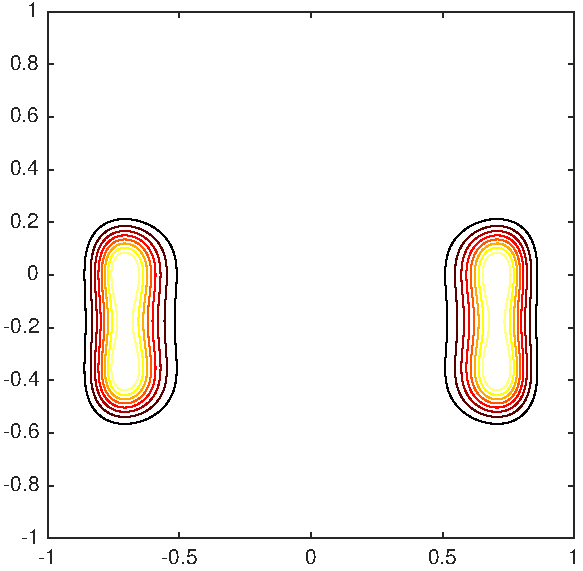
\includegraphics[width=0.7\columnwidth]{chebfun2.pdf}}%
	\only<3>{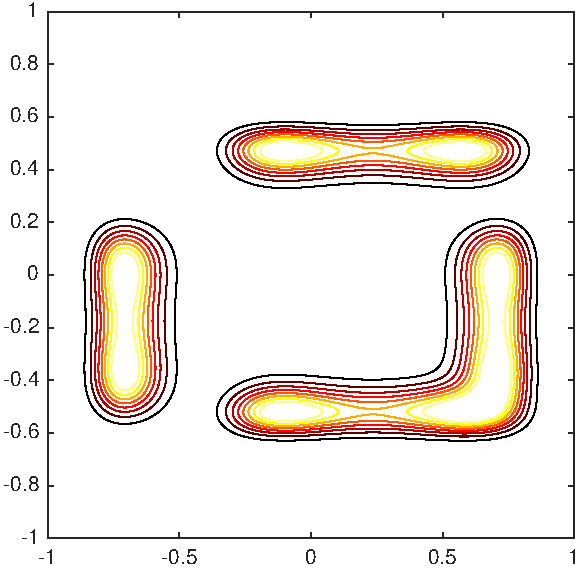
\includegraphics[width=0.7\columnwidth]{chebfun3.pdf}}%
	\only<4>{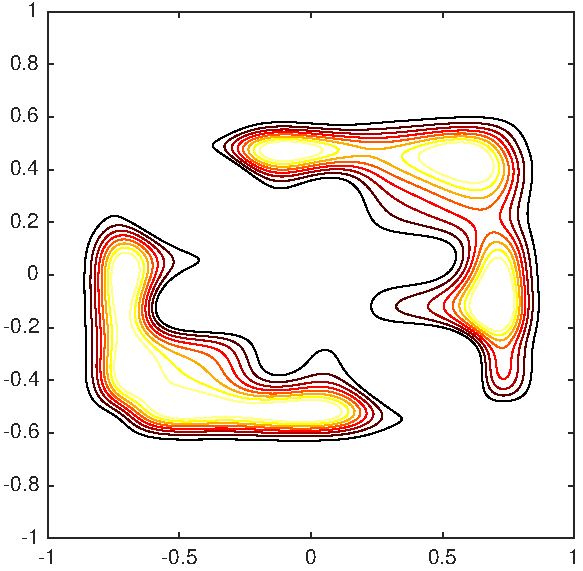
\includegraphics[width=0.7\columnwidth]{chebfun4.pdf}}%
	\only<5>{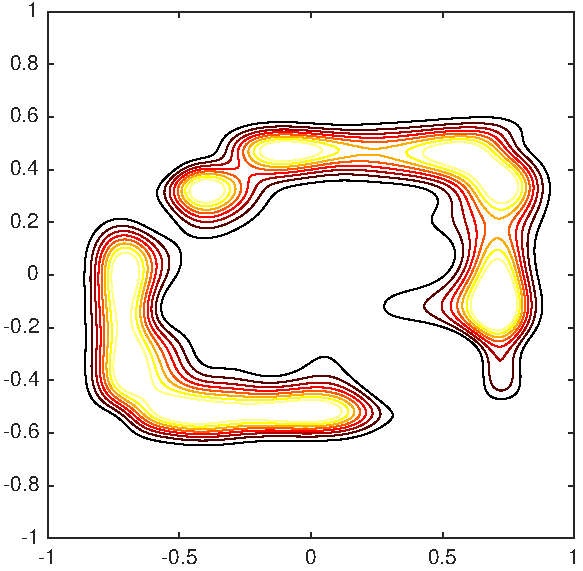
\includegraphics[width=0.7\columnwidth]{chebfun5.pdf}}%
	\only<6>{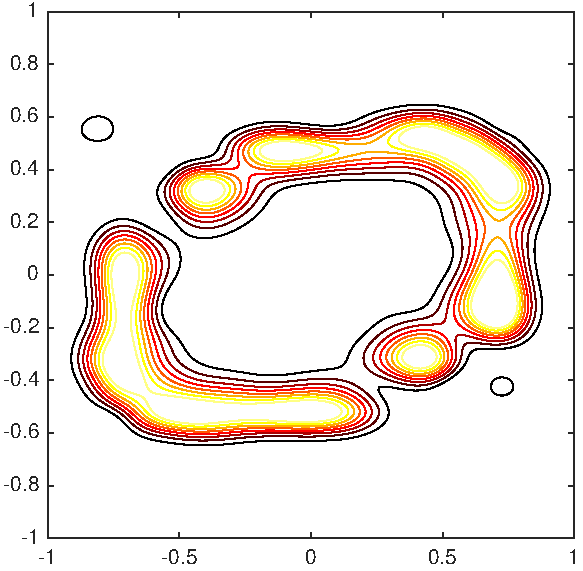
\includegraphics[width=0.7\columnwidth]{chebfun6.pdf}}%
	\only<7>{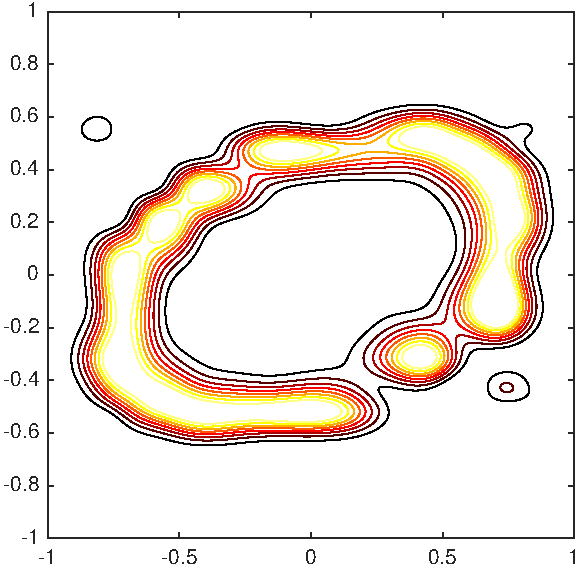
\includegraphics[width=0.7\columnwidth]{chebfun7.pdf}}%
	\only<8>{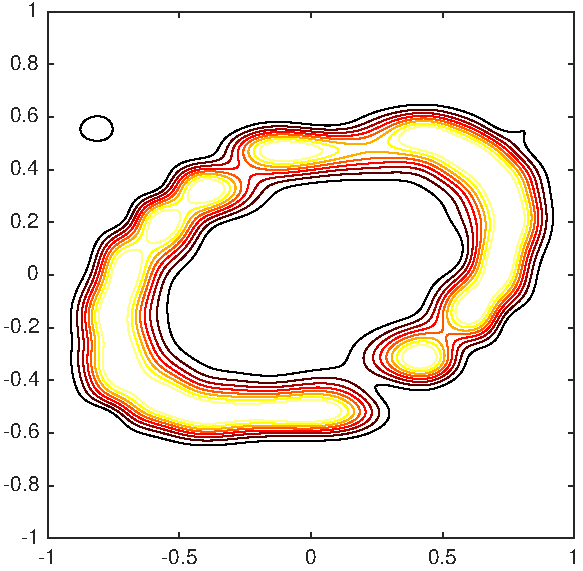
\includegraphics[width=0.7\columnwidth]{chebfun8.pdf}}%
	\only<9>{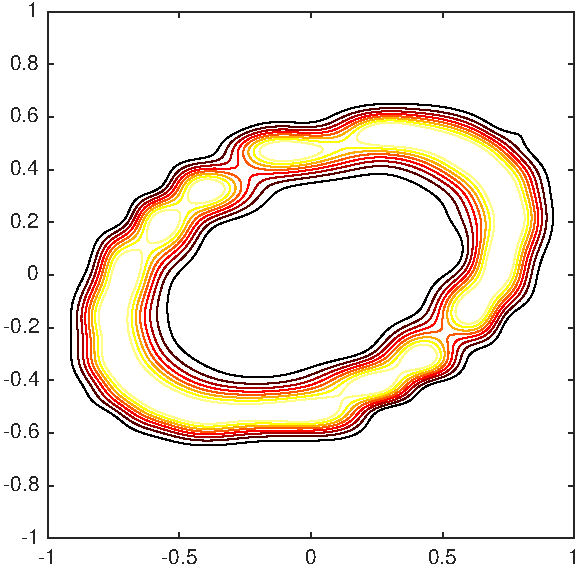
\includegraphics[width=0.7\columnwidth]{chebfun9.pdf}}%
	\only<10>{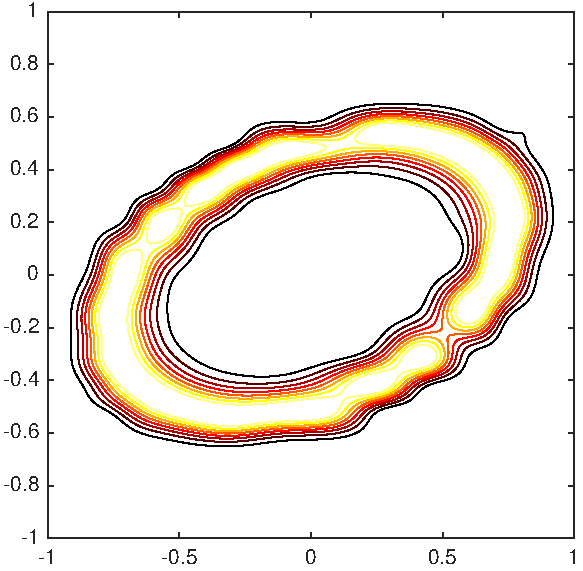
\includegraphics[width=0.7\columnwidth]{chebfun10.pdf}}
\end{column}
\end{columns}
\end{onlyenv}
\only<11>{
\[
F = (f(x_i,x_j))_{i,j} \qquad \operatorname{rank}(F) = \vcenter{\hbox{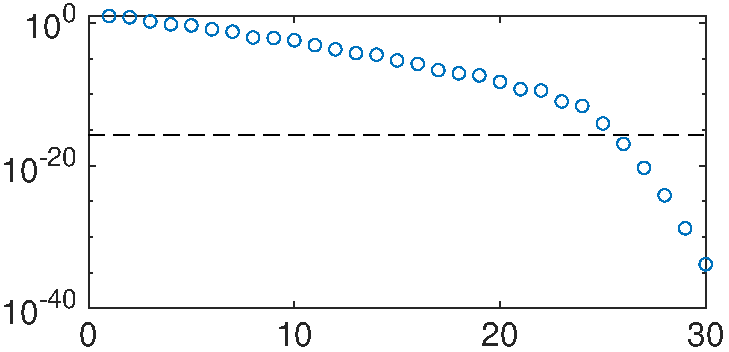
\includegraphics[width=0.5\columnwidth]{chebfunsvd.pdf}}} \approx 25.
\]
}

	\end{frame}

	\begin{frame}{Low-rank, regularity and separability}
	\begin{itemize}
		\item[\faEye]<1-> Not every right-hand side will have a small-enough rank!
		\item[\faHammer]<2-> Whenever we have \textbf{closed form expression} of the \textbf{involved functions} we can work with polynomial basis expansion to discover the rank.
		\item[\faCog]<3-> To actually compute the decomposition $C = C_1 C_2^H$ we need we can either
		\begin{itemize}
			\item[\faBomb]<4-> \normalsize assemble everything and use the \textbf{SVD},
			\item[\faHammer]<5-> \normalsize work with \textbf{polynomial expansion} and truncate it for small enough coefficients, e.g., \parencite{carvajal2005hybrid,MR3138114,MR3947283},
			\item[\faBarcode]<6-> \normalsize using algorithm that only need to compute \emph{few} entries of $A$, such as Adaptive-Cross-Approximation~\parencite{MR1783468}, or RandSVD-type algorithms~\parencite{MR2806637}.
		\end{itemize}
	\end{itemize}
	
	\begin{block}<7>{\faExclamationCircle\;\;Approximating approximating we could get where we wanted$\ldots$}
	Let us remember that the approximation of the low-rank term must be done together with the approximation induced by the FDE solution method. We may not need to go as far as machine precision.
	\end{block}
	
	\end{frame}

	\subsection{Selecting the Krylov subspace}
	
	\begin{frame}{Selecting the Krylov subspace}
	If we are now in the case of a \textbf{low rank} right-hand side, we have to select Krylov subspaces for the spaces $\mathcal{V}$ and $\mathcal{W}$.
	
	\begin{itemize}
		\item[\faExclamationCircle]<1-> From the work we have done in the last couple of lectures, we know how to solve linear systems involving discretization of 1D problems,
		\item[\textcolor{Goldenrod}{\faLightbulb}]<2-> Rational (block) Krylov subspace can therefore be a good choice!
		\[ 
		\begin{split}
			\mathcal{V} = &\;\operatorname{range}\{[ (A+ \sigma_1 I)^{-1} C_1, (A+ \sigma_2 I)^{-1} (A+ \sigma_1 I)^{-1} C_1,\ldots] \}, \\ \mathcal{W} = &\; \operatorname{range}\{[ (B^H + \eta_1 I)^{-1} C_2, (B^H+ \eta_2 I)^{-1} (B^H+ \eta_1 I)^{-1} C_2,\ldots] \},
		\end{split}
		\]
		\item[\faQuestionCircle]<3-> $\ldots$ but how do we \textbf{select the poles}?
		\item[\alert{\faExclamationTriangle}]<4-> This is not an easy problem in general! A maybe lazy (but surprisingly well behaving) choice is to set $\{\sigma_i,\eta_i\} \in \{0,\infty\}$ $\Rightarrow$ if we choose the two values alternately, then we get the \alert{Extended Krylov Subspace}.
	\end{itemize}
	
	\end{frame}

	\begin{frame}{The Extended Krylov Subspace approach}
	If $B = A^T$ and $C = C_1 C_2^T$ with $C_1 = C_2$, we can generate the space:
	\[
	\mathbb{EK}(A,C_1) = \operatorname{range}([C_1,A^{-1}C_1,AC_1,A^{-2}C_1,A^2C_1,\ldots]) = \mathcal{V} = \mathcal{W}.
	\]
	The resulting algorithm is the KPIK method by~\parencite{MR2318706}, and can be easily extended to solve the general case, by building both
	\[
	\begin{split}
	\mathcal{V} = & \;\mathbb{EK}(A,C_1) = \operatorname{range}([C_1,A^{-1}C_1,AC_1,A^{-2}C_1,A^2C_1,\ldots]),\\
	\mathcal{W} = & \;\mathbb{EK}(B^T,C_2) = \operatorname{range}([C_2,B^{-T}C_2,B^TC_2,A^{-2T}C_2,A^{2T}C_2,\ldots]).
	\end{split}
	\]
	\onslide<2>{
	For our two problems, we have to solve systems and do mat-vec with matrices
	\begin{align*}
		\text{1D: } & A = \frac{-\Delta t}{h_N^\alpha} ( \theta G_N + (1-\theta) G_N^T) & B = & T_M(1-e^{i\theta}) \\
		\text{2D: } & A = \frac{1}{2} I_{N_x} - \frac{\Delta t}{h_{N_x}^\alpha} ( \theta G_{N_x} + (1-\theta) G_{N_x}^T) & B = & \frac{1}{2} I_{N_y} - \frac{\Delta t}{h_{N_y}^\alpha} ( \theta G_{N_y} + (1-\theta) G_{N_y}^T) \\
	\end{align*}
	}
	
	\end{frame}

	\begin{frame}[fragile]{A couple of examples - I}
	Let us start from the 1D+1D case
	\[
	\begin{cases}
	\frac{\partial W}{\partial t} = \Gamma(3-\alpha) x^\alpha\, {}^{RL}D_{[0,x]}^\alpha W + \Gamma(3-\alpha) (2-x)^\alpha {}^{RL}D_{[x,2]}^\alpha W - x(x-2)e^{-t},\\
	W(0,t) = W(1,t) = 0, \quad W(x,0) = 5x(2-x);
	\end{cases}
	\]
	We can \textbf{discretize it} in the usual way:\vspace{-1em}
\begin{columns}
\begin{column}{0.55\columnwidth}
\definecolor{bg}{rgb}{0.95,0.95,0.95}
\begin{minted}[bgcolor=bg,fontsize=\small,breaklines]{matlab}
w0 = @(x) 5*x.*(2-x);
hN = 2/(N-1); x = 0:hN:2;
dt = hN; t = 0:dt:1; M = length(t);
dplus=@(x,t)gamma(3-alpha).*x.^alpha;
dmin=@(x,t)gamma(3-alpha).*(2-x).^alpha;
f= @(x,t) -x.*(x-2).*exp(-t);
G = glmatrix(N,alpha);
Gr = G; Grt = G.';
Dplus = diag(dplus(x,0));
Dminus = diag(dmin(x,0));
I = eye(N,N); e = ones(N,1);
\end{minted}
\end{column}
\begin{column}{0.45\columnwidth}
\definecolor{bg}{rgb}{0.95,0.95,0.95}
\begin{minted}[bgcolor=bg,fontsize=\small,breaklines]{matlab}
A = -dt*(Dplus*Gr + Dminus*Grt)/hN^alpha;
B = spdiags([-e,e],-1:0,M,M);
[X,T] = meshgrid(x,t);
C = dt*f(X,T);
C(1,:) = w0(x) + C(1,:);
C = -C';
[U,S,V] = svd(C);
C1 = U(:,1:2)*sqrt(S(1:2,1:2));
C2 = (sqrt(S(1:2,1:2))* V(:,1:2).').';
\end{minted}
\end{column}
\end{columns}

	\end{frame}

\begin{frame}[fragile]{A couple of examples - I}
And then use the \texttt{kpik\_sylv} solver from \href{http://www.dm.unibo.it/~simoncin/software.html}{V. Simoncini's software}:
\begin{columns}
\begin{column}{0.5\columnwidth}
\definecolor{bg}{rgb}{0.95,0.95,0.95}
\begin{minted}[bgcolor=bg,fontsize=\small,breaklines]{matlab}
m = 100;
tol = 1e-9;
[LA,UA] = lu(A); % Direct solutions!
[LB,UB] = lu(B);
[X1,X2,res]=kpik_sylv(A,LA,UA, B,LB,UB,C1,C2,m,tol);
SOL = X1*X2'; % Not clever al all!
\end{minted}
\begin{itemize}
	\item[\alert{\faExclamationTriangle}] We are using LU-factorization and direct solutions;
	\item[\alert{\faExclamationTriangle}] We are reassembling the solution!
\end{itemize}
\end{column}
\begin{column}{0.5\columnwidth}

\only<1>{\centering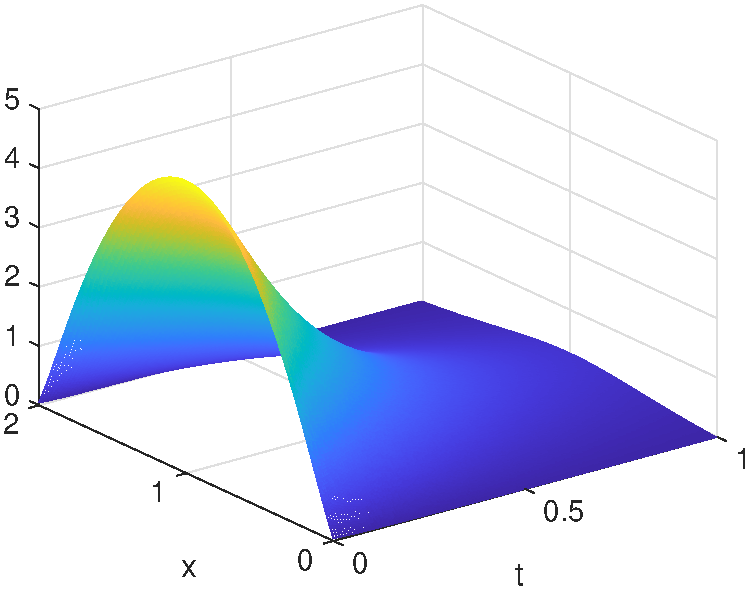
\includegraphics[width=\columnwidth]{sylv_sol.pdf}
	
	$N = 2^8$, $M = 2^7$, $\alpha = 1.5$
}%

\begin{onlyenv}<2>
\centering

\begin{tabular}{cccc}
\toprule
$\alpha$ & $N = 2M$ & IT & Rel. Residual \\
\midrule
 1.2 & $2^{5}$ & 7 & 4.982093e-10 \\
& $2^{6}$ & 11 & 7.629176e-11 \\
& $2^{7}$ & 15 & 3.721767e-10 \\
& $2^{8}$ & 21 & 2.406077e-10 \\
& $2^{9}$ & 28 & 4.726518e-10 \\
& $2^{10}$ & 37 & 8.250742e-10 \\
& $2^{11}$ & 50 & 5.928325e-10 \\
\bottomrule
\end{tabular}

\end{onlyenv}
\begin{onlyenv}<3>
	\centering
	
	\begin{tabular}{cccc}
		\toprule
		$\alpha$ & $N = 2M$ & IT & Rel. Residual \\
		\midrule
 1.3 & $2^{5}$ & 8 & 7.473189e-41 \\
& $2^{6}$ & 10 & 3.324155e-10 \\
& $2^{7}$ & 14 & 1.876221e-10 \\
& $2^{8}$ & 18 & 6.104754e-10 \\
& $2^{9}$ & 24 & 4.098504e-10 \\
& $2^{10}$ & 31 & 5.142375e-10 \\
& $2^{11}$ & 40 & 6.702602e-10 \\
\bottomrule
\end{tabular}

\end{onlyenv}
\begin{onlyenv}<4>
	\centering
	
	\begin{tabular}{cccc}
		\toprule
		$\alpha$ & $N = 2M$ & IT & Rel. Residual \\
		\midrule
 1.4 & $2^{5}$ & 7 & 4.900654e-10 \\
& $2^{6}$ & 10 & 4.402728e-11 \\
& $2^{7}$ & 13 & 1.970841e-10 \\
& $2^{8}$ & 17 & 2.024635e-10 \\
& $2^{9}$ & 22 & 5.120085e-10 \\
& $2^{10}$ & 28 & 8.263324e-10 \\
& $2^{11}$ & 36 & 8.596848e-10 \\
\bottomrule
\end{tabular}

\end{onlyenv}
\begin{onlyenv}<5>
	\centering
	
	\begin{tabular}{cccc}
		\toprule
		$\alpha$ & $N = 2M$ & IT & Rel. Residual \\
		\midrule
1.5 & $2^{5}$ & 7 & 1.235969e-10 \\
& $2^{6}$ & 9 & 2.799035e-10 \\
& $2^{7}$ & 13 & 1.007848e-10 \\
& $2^{8}$ & 16 & 6.145733e-10 \\
& $2^{9}$ & 21 & 7.639171e-10 \\
& $2^{10}$ & 27 & 5.857467e-10 \\
& $2^{11}$ & 34 & 8.065585e-10 \\
\bottomrule
\end{tabular}

\end{onlyenv}
\begin{onlyenv}<6>
	\centering
	
	\begin{tabular}{cccc}
		\toprule
		$\alpha$ & $N = 2M$ & IT & Rel. Residual \\
		\midrule
1.6 & $2^{5}$ & 7 & 2.480357e-11 \\
& $2^{6}$ & 9 & 8.683894e-11 \\
& $2^{7}$ & 13 & 7.692141e-11 \\
& $2^{8}$ & 16 & 3.792143e-10 \\
& $2^{9}$ & 21 & 3.991222e-10 \\
& $2^{10}$ & 26 & 6.017048e-10 \\
& $2^{11}$ & 33 & 6.133773e-10 \\
\bottomrule
\end{tabular}

\end{onlyenv}
\begin{onlyenv}<7>
	\centering
	
	\begin{tabular}{cccc}
		\toprule
		$\alpha$ & $N = 2M$ & IT & Rel. Residual \\
		\midrule
1.7 & $2^{5}$ & 7 & 5.588528e-12 \\
& $2^{6}$ & 8 & 6.692127e-10 \\
& $2^{7}$ & 12 & 8.189936e-10 \\
& $2^{8}$ & 16 & 3.403250e-10 \\
& $2^{9}$ & 20 & 9.093120e-10 \\
& $2^{10}$ & 26 & 3.550244e-10 \\
& $2^{11}$ & 32 & 7.478792e-10 \\
\bottomrule
\end{tabular}

\end{onlyenv}
\begin{onlyenv}<8>
	\centering
	
	\begin{tabular}{cccc}
		\toprule
		$\alpha$ & $N = 2M$ & IT & Rel. Residual \\
		\midrule
1.8 & $2^{5}$ & 6 & 6.097527e-10 \\
& $2^{6}$ & 8 & 9.737670e-11 \\
& $2^{7}$ & 13 & 6.202872e-11 \\
& $2^{8}$ & 16 & 2.193864e-10 \\
& $2^{9}$ & 20 & 7.469866e-10 \\
& $2^{10}$ & 25 & 8.191797e-10 \\
& $2^{11}$ & 32 & 5.086938e-10 \\
\bottomrule
\end{tabular}

\end{onlyenv}
\only<9>{
\centering

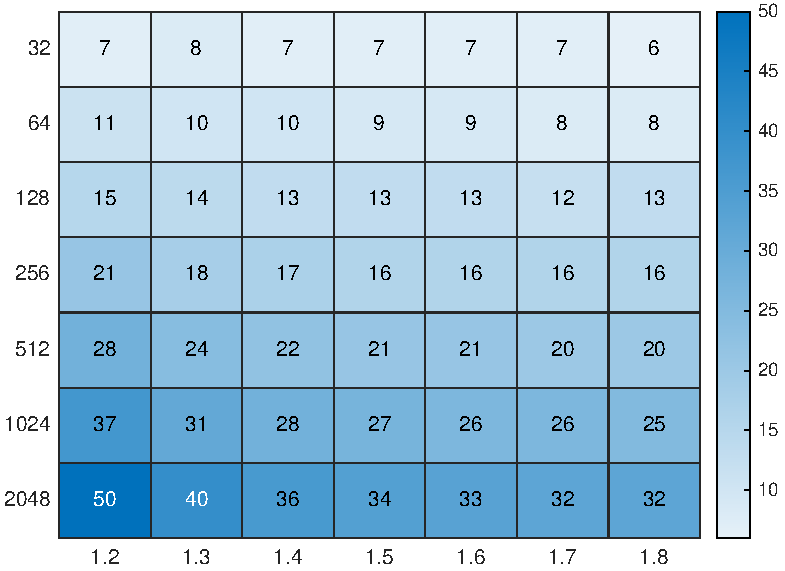
\includegraphics[width=\columnwidth]{sylvsolvit.pdf}
}
\end{column}
\end{columns}
\end{frame}

	\begin{frame}[fragile]{A couple of examples - II}
	We can then try the 1D+2D case
	\[
	\begin{cases}
	\frac{\partial W}{\partial t} = \Gamma(3-\alpha) x^\alpha\, {}^{RL}D_{[0,x]}^\alpha W + \Gamma(3-\alpha) (2-x)^\alpha {}^{RL}D_{[x,2]}^\alpha W  \\
	\phantom{\frac{\partial W}{\partial t} = } + \Gamma(3-\alpha) y^\alpha\, {}^{RL}D_{[0,y]}^\alpha W + \Gamma(3-\alpha) (2-y)^\alpha {}^{RL}D_{[y,2]}^\alpha W \\
	\phantom{\frac{\partial W}{\partial t} = } + \sin(\pi x) \sin(\pi y) e^{-t},\\
	W(x,y,t) =  0, & (x,y) \in \partial [0,2]^2,\\
	W(x,y,0) = 5x(2-x)y(2-y),
	\end{cases}
	\]
	for which the discretization proceeds along the usual lines, i.e,\vspace{-0.7em}
	\begin{onlyenv}<1>
	\definecolor{bg}{rgb}{0.95,0.95,0.95}
\begin{minted}[bgcolor=bg,fontsize=\small,breaklines]{matlab}
hN = 2/(N-1); x = 0:hN:2; y = 0:hN:2; [X,Y] = meshgrid(x,y);
dt = hN; t = 0:dt:1; M = length(t);
w0 = @(x,y) 5*x.*(2-x).*y.*(2-y);
dplus = @(x,t) gamma(3-alpha).*x.^alpha;
dminus = @(x,t) gamma(3-alpha).*(2-x).^alpha;
f = @(x,y,t) sin(pi*x).*sin(pi*y).*exp(-t);
\end{minted}
	\end{onlyenv}
\begin{onlyenv}<2>
\definecolor{bg}{rgb}{0.95,0.95,0.95}
\begin{minted}[bgcolor=bg,fontsize=\small,breaklines]{matlab}
G = glmatrix(N,alpha); Gr = G; Grt = G.';
Dplus = diag(dplus(x,0)); Dminus = diag(dminus(x,0));
I = eye(N,N); e = ones(N,1);
A = 0.5*I -dt*(Dplus*Gr + Dminus*Grt)/hN^alpha; % Left-hand side
B = (0.5*I -dt*(Dplus*Gr + Dminus*Grt)/hN^alpha).';
C = w0(X,Y) + dt*f(X,Y,t(1)); C = -C'; [U,S,V] = svd(C);  % Right-hand side
C1 = U(:,1:2)*sqrt(S(1:2,1:2)); C2 = (sqrt(S(1:2,1:2))*V(:,1:2).').';
\end{minted}
\end{onlyenv}
	\end{frame}

\begin{frame}[fragile]{A couple of examples - II}
And then use the \texttt{kpik\_sylv} solver from \href{http://www.dm.unibo.it/~simoncin/software.html}{V. Simoncini's software}:
\begin{columns}
	\begin{column}{0.5\columnwidth}
		\definecolor{bg}{rgb}{0.95,0.95,0.95}
		\begin{minted}[bgcolor=bg,fontsize=\small,breaklines]{matlab}
m = 100;
tol = 1e-9;
[LA,UA] = lu(A); % Direct solutions!
[LB,UB] = lu(B);
[X1,X2,res]=kpik_sylv(A,LA,UA, B,LB,UB,C1,C2,m,tol);
SOL = X1*X2'; % Not clever al all!
		\end{minted}
		\begin{itemize}
			\item[\alert{\faExclamationTriangle}] We are using LU-factorization and direct solutions;
			\item[\alert{\faExclamationTriangle}] We are reassembling the solution!
		\end{itemize}
	\end{column}
	\begin{column}{0.5\columnwidth}
		
		\only<1>{\centering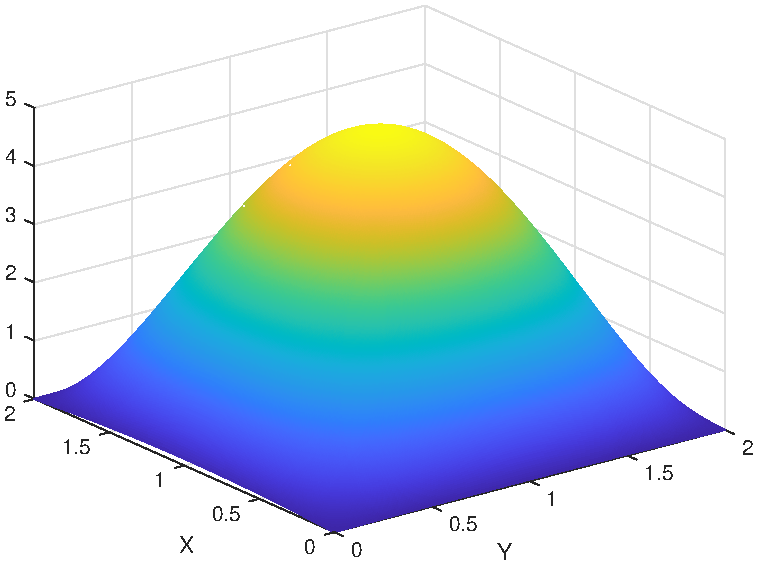
\includegraphics[width=\columnwidth]{sylv_sol2.pdf}
			
			$N = 2^8$, $M = 2^8$, $\alpha = 1.5$
		}%
		
		\begin{onlyenv}<2>
			\centering
			
			\begin{tabular}{cccc}
				\toprule
				$\alpha$ & $N = M$ & IT & Rel. Residual \\
				\midrule
 1.2 & $2^{5}$ & 7 & 8.572314e-12 \\
& $2^{6}$ & 9 & 1.035235e-10 \\
& $2^{7}$ & 10 & 6.376925e-10 \\
& $2^{8}$ & 11 & 4.294848e-10 \\
& $2^{9}$ & 11 & 4.831316e-10 \\
& $2^{10}$ & 11 & 3.340377e-10 \\
& $2^{11}$ & 10 & 8.493637e-10 \\
				\bottomrule
			\end{tabular}
			
		\end{onlyenv}
		\begin{onlyenv}<3>
			\centering
			
			\begin{tabular}{cccc}
				\toprule
				$\alpha$ & $N = M$ & IT & Rel. Residual \\
				\midrule
 1.3 & $2^{5}$ & 7 & 7.117681e-11 \\
& $2^{6}$ & 9 & 7.410001e-11 \\
& $2^{7}$ & 10 & 6.311608e-10 \\
& $2^{8}$ & 11 & 6.629092e-10 \\
& $2^{9}$ & 11 & 7.935697e-10 \\
& $2^{10}$ & 11 & 5.256769e-10 \\
& $2^{11}$ & 11 & 3.021361e-10 \\
				\bottomrule
			\end{tabular}
			
		\end{onlyenv}
		\begin{onlyenv}<4>
			\centering
			
			\begin{tabular}{cccc}
				\toprule
				$\alpha$ & $N = M$ & IT & Rel. Residual \\
				\midrule
 1.4 & $2^{5}$ & 7 & 6.199844e-11 \\
& $2^{6}$ & 9 & 5.440959e-11 \\
& $2^{7}$ & 10 & 6.223106e-10 \\
& $2^{8}$ & 12 & 2.743756e-10 \\
& $2^{9}$ & 12 & 6.270319e-10 \\
& $2^{10}$ & 12 & 4.310692e-10 \\
& $2^{11}$ & 11 & 4.849822e-10 \\
				\bottomrule
			\end{tabular}
			
		\end{onlyenv}
		\begin{onlyenv}<5>
			\centering
			
			\begin{tabular}{cccc}
				\toprule
				$\alpha$ & $N = M$ & IT & Rel. Residual \\
				\midrule
 1.5 & $2^{5}$ & 7 & 5.108938e-11 \\
& $2^{6}$ & 8 & 7.696608e-10 \\
& $2^{7}$ & 10 & 5.554438e-10 \\
& $2^{8}$ & 12 & 3.501633e-10 \\
& $2^{9}$ & 13 & 4.696907e-10 \\
& $2^{10}$ & 13 & 5.839644e-10 \\
& $2^{11}$ & 12 & 6.172378e-10 \\
				\bottomrule
			\end{tabular}
			
		\end{onlyenv}
		\begin{onlyenv}<6>
			\centering
			
			\begin{tabular}{cccc}
				\toprule
				$\alpha$ & $N = M$ & IT & Rel. Residual \\
				\midrule
 1.6 & $2^{5}$ & 7 & 4.147318e-11 \\
& $2^{6}$ & 9 & 1.120891e-10 \\
& $2^{7}$ & 10 & 4.652358e-10 \\
& $2^{8}$ & 12 & 3.624143e-10 \\
& $2^{9}$ & 13 & 6.835564e-10 \\
& $2^{10}$ & 14 & 5.920602e-10 \\
& $2^{11}$ & 13 & 8.882506e-10 \\
				\bottomrule
			\end{tabular}
			
		\end{onlyenv}
		\begin{onlyenv}<7>
			\centering
			
			\begin{tabular}{cccc}
				\toprule
				$\alpha$ & $N = M$ & IT & Rel. Residual \\
				\midrule
 1.7 & $2^{5}$ & 7 & 3.321348e-11 \\
& $2^{6}$ & 9 & 9.437180e-11 \\
& $2^{7}$ & 10 & 7.551800e-10 \\
& $2^{8}$ & 12 & 3.268160e-10 \\
& $2^{9}$ & 13 & 7.715645e-10 \\
& $2^{10}$ & 14 & 8.954668e-10 \\
& $2^{11}$ & 15 & 5.806398e-10 \\
				\bottomrule
			\end{tabular}
			
		\end{onlyenv}
		\begin{onlyenv}<8>
			\centering
			
			\begin{tabular}{cccc}
				\toprule
				$\alpha$ & $N = M$ & IT & Rel. Residual \\
				\midrule
 1.8 & $2^{5}$ & 7 & 2.639521e-11 \\
& $2^{6}$ & 9 & 7.654578e-11 \\
& $2^{7}$ & 10 & 6.909946e-10 \\
& $2^{8}$ & 12 & 4.424195e-10 \\
& $2^{9}$ & 13 & 7.255110e-10 \\
& $2^{10}$ & 15 & 4.728355e-10 \\
& $2^{11}$ & 15 & 8.400505e-10 \\
				\bottomrule
			\end{tabular}
			
		\end{onlyenv}
		\only<9>{
			\centering
			
			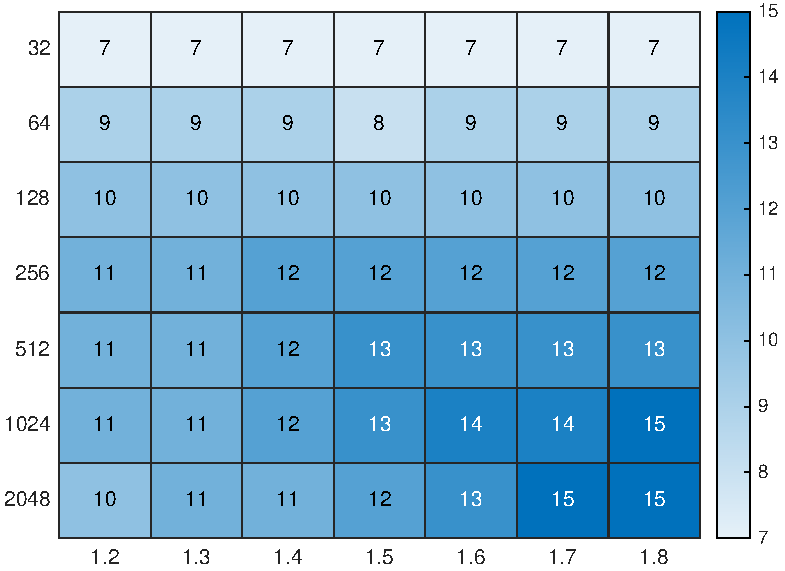
\includegraphics[width=\columnwidth]{sylvsolvit2.pdf}
		}
	\end{column}
\end{columns}
\end{frame}

	\subsection{Convergence}
	
	\begin{frame}{Convergence}
	\faQuestionCircle\;What can we say about the convergence?
	\vfill
	
	\onslide<2->{\faCogs\;If $A$ is symmetric and positive definite, and $B = A^T$, i.e., we are solving a Lyapunov equation, and using \textbf{polynomial Krylov subspace}:
	\begin{alertblock}{Theorem \parencite[Proposition~3.1]{MR2485434}}
	Let $A$ be symmetric and positive definite, and let $\lambda_{\min}$ be the smallest eigenvalue of $A$. Let $\hat{\lambda}_{\min}$, $\hat{\lambda}_{\max}$ be the extreme eigenvalue of $A + \lambda_{\min} I$ and $\hat{\kappa} = \nicefrac{\hat{\lambda}_{\max}}{\hat{\lambda}_{\min}}$. Then
	\[
	\|X - X_m\| \leq 4 \frac{\sqrt{\hat{\kappa}} + 1}{\hat{\lambda}_{\min} \sqrt{\hat{\kappa}}} \left( \frac{\sqrt{\hat{\kappa}} - 1}{\sqrt{\hat{\kappa}} + 1} \right)^m.
	\]
	\end{alertblock}}
	\vfill

	\onslide<3>{\alert{\faExclamationTriangle}\;If $B = A^T$ but $A$ is \textbf{no longer symmetric}, one then needs again bounds related to the Field-of-Values of $A$, see \parencite{MR2485434}.} 
	\end{frame}

	\begin{frame}{Convergence}
	If we have $B \neq A^T$ things are more involved and due to \parencite{MR2854603}, and we need preliminary work.
	\begin{itemize}
		\item[\faBook] First of all, we need a more manageable expression of the rational Krylov subspace, let us re-brand the poles in the extended complex plane $\overline{\mathbb{C}} = \mathbb{C} \cup \{\infty\}$ as
		\[
		z_{A,1},\ldots,z_{A,m} \in \overline{\mathbb{C}} \setminus \Lambda(A), \qquad z_{B,1},\ldots,z_{B,n} \in \overline{\mathbb{C}} \setminus \Lambda(B),
		\] 
		and introduce the polynomials 
		\[Q_A(z) = \prod_{\substack{j=1\\z_{A,j} \neq \infty}}^m (z-z_{A,j}) \text{ and }Q_B(z) = \prod_{\substack{j=1\\z_{B,j} \neq \infty}}^n (z-z_{A,j}).\]
		\item[\faBook]<2-> The two rational spaces can then be written as
		\[
		\mathcal{V} = \{ R_A(A)C_1 \,:\; R_A \in \mathbb{P}_{m-1}/Q_A \}, \qquad \mathcal{W} = \{ R_B(B)^H C_2 \,:\; R_B \in \mathbb{P}_{n-1}/Q_B \}.
		\]
	\end{itemize}
	
	\end{frame}

	\begin{frame}{Convergence}
	\begin{itemize}
		\item[\faWrench] Consider the \textbf{rational functions} for the projected matrices $A_m$ and $B_n$ on $\mathcal{V}$ and~$\mathcal{W}$
		\[
		R_A^G(z) = \frac{\det(zI - A)}{Q_A(z)} \in \mathbb{P}_{m}/Q_A, \qquad R_B^G(z) = \frac{\det(zI - B_n)}{Q_B(z)} \in \mathbb{P}_n/Q_B
		\]
	\end{itemize}
	\vspace{-0.8em}\only<2-5>{\begin{alertblock}<2->{Theorem \parencite[Theorem~2.1]{MR2854603}}
	Let $\operatorname{rank}(C) = 1$. The rational Galerkin residual $\rho$ can be decomposed into the sum\hspace{-1.2em}
	\[
	\rho = \rho_{1,2} + \rho_{2,1} + \rho_{2,2}, \qquad \|\rho\|_F^2 = \|\rho_{1,2}\|_F^2 + \|\rho_{2,1}\|_F^2 + \|\rho_{2,2}\|_F^2,
	\]
	with, $C_{1,m} = U^H C_1$, $C_{2,n} = V^H C_2$, and\hspace{-0.7em}
	\only<2>{\begin{gather*}
	\rho_{1,2} U \frac{1}{R^G_B}(A_m) C_{1,m} C_2^H R_B^G(B), \;\; \rho_{2,1} = R_A^G(A) C_1 C_{2,n}^H \frac{1}{R_A^G}(B_n)V^H, \\
	\rho_{2,2} = \frac{R_A^G(A)C_1C_2^H R_B^G(B)}{R_A^G(\infty)R_B^G(\infty)}.
	\end{gather*}}%
	\only<3>{
	\begin{equation*}
	\|\rho_{2,2}\|_F = \inf_{ \substack{ R_A \in \mathbb{P}_m/Q_A \\ R_B \in \mathbb{P}_n/Q_B } } \left\| \frac{R_A(A)C_1C_2^H R_B(B)}{R_A(\infty)R_B(\infty)} \right\|_F = \| (I-UU^H) C_1 C_2^H (I - VV^H) \|_F,
	\end{equation*}
	}%
	\only<4>{
	\[
	\| \rho_{1,2}\|_F = \min_{R_B \in \mathbb{P}_m/Q_B} \left[ \| R_B(A_m) C_{1,m} C_{2}^H R_B(B)\|_F + c_0 \| \frac{1}{R_B}(A_m) C_{1,m} C_{2,n}^H R_B(B_n) \|_F \right],
	\]
	for $c_0 = 2 \operatorname{diam}(W(A),W(B))/\operatorname{dist}(W(A),W(B))$.
	}%
	\only<5>{
	\[
	\| \rho_{2,1}\|_F = \min_{R_A \in \mathbb{P}_m/Q_A} \left[ \| R_A(A) C_1 C_{2,n}^H \frac{1}{R_A}(B_n)\|_F + c_0 \| R_A(A_m) C_{1,m} C_{2,n}^H \frac{1}{R_A}(B_n) \|_F \right],
	\]
	for $c_0 = 2 \operatorname{diam}(W(A),W(B))/\operatorname{dist}(W(A),W(B))$.
	}%
	\end{alertblock}}%
	\only<6->{
	\begin{itemize}
		\item[\faWrench] Now we have a \textbf{representation of the residual} in the \textbf{orthogonal bases} associated to the given Krylov subspaces, and furthermore we know that $\rho_{2,2} = 0$ if at least one of the $z_{A,j}$ or $z_{B,j}$ is $\infty$, i.e., if either of the initial vectors are in the subspace.
		\item[\faCog]<7-> The bounds are then obtained by having upper-bounds of the quantities
		\[
		E_m(\spadesuit,Q_\spadesuit,z) = \min_{p \in \mathbb{P}_\heartsuit} \frac{\left\| \frac{P}{Q_\spadesuit}(\spadesuit) \right\|}{\left\lvert \frac{P}{Q_\spadesuit}(z) \right\rvert}, \text{ for } \spadesuit = \{A,B\}, \; \heartsuit = \{m,n\}.
		\]
		\item[$\Rightarrow$]<8-> This can be faced by using the upper bound given by \alert{Crouziex upper-bound for matrix-functions}.
	\end{itemize}
	}
	\end{frame}

	\begin{frame}{Convergence: potential theory}
	
	\faHammer\; In order to obtain the bounds and the rate of convergence, we need to work with the \textbf{Green functions} of $\overline{\mathbb{C}}\setminus W(A)$ and $\overline{\mathbb{C}}\setminus W(B)$ with poles at $\zeta \in \mathbb{C}$ called $g_A(\cdot,\zeta)$ and $g_B(\cdot,\zeta)$ respectively; \parencite{MR1485778}. 
	
	\onslide<2->{\vfill
	With this \textbf{potential functions} the bound can then be expressed in terms of the functions
	\[
	u_{A,m}(z) = \exp \left( - \sum_{j=1}^{m} g_A(z,z_{A,j})\right), \text{ and } u_{B,n}(z) = \exp \left( - \sum_{j=1}^{n} g_B(z,z_{B,j})\right).
	\]
	}
	
	\vfill
	\begin{exampleblock}<3->{\faBinoculars\;A mad research idea}
	Given the case we are interested in, can we find \textbf{optimal poles}, i.e., the one minimizing the bounds and have both $\alpha$ robustness, and $M$ and $N$ independence? 
	\end{exampleblock}
	
	\end{frame}

	\subsection{Let's blow up the bridges}
	
	\begin{frame}{\faBomb\;Let's blow up the bridges}
		
	\faQuestionCircle\;What do we do if the \textbf{space coefficients} are \textbf{not separable}?
	\begin{itemize}
		\item[\faCog]<2-> We decompose
		\[
			d^{\pm}(x,y) = \sum_{k=1}^{K} t_k^{\pm} T_k(x)T_k(y)
		\]
		and substitute in our equation obtaining
		\[
		\sum_{k=1}^{K} \left( \tilde{A}_k X + X\tilde{B}^T_k \right) = C_1C_2^T. 
		\]
		\item[\faHammer]<3-> We can try generalize the Galerkin projection 
		\[
		\sum_{k=1}^{2K} \hat{A}_k X \hat{B}_k = C_1C_2^T \;\Rightarrow\; \sum_{k=1}^{2K} (V_m^T \hat{A}_k V_m ) X ( W_m^T \hat{B}_k W_m ) = V_m C_1 (W_m^T C_2)^T,
		\]
		\begin{itemize}
			\item[\faCog]<4-> How do we select $\mathcal{V}$ and $\mathcal{W}$? How do we generate nested subspace? How do we solve the reduced multiterm equation? \onslide<5->{ $\Rightarrow$ many more questions than answers$\ldots$ \alert{\faSadTear}.}
		\end{itemize}
	\end{itemize}

	\end{frame}

	\begin{frame}{\faBomb\;Let's blow up the bridges}
	\onslide<1->{\faQuestionCircle\;What if the \textbf{convergence rate} is \textbf{poor}?}
	\begin{itemize}
		\item[\only<2>{\faLightbulb}\only<5>{\alert{\faSadCry}}]<4-> Since convergence depends on the spectrum, we may be tempted to precondition the equation with a matrix $P$, i.e.,
		\[
		\only<2>{P^{-1}AXP^{-H} + P^{-1} X B P^{-H} = P^{-1} C P^{-H},}
		\only<3->{(P^{-1}AP)P^{-1}XP^{-H} + P^{-1}XP^{-H} (P^H B P^{-H}) = P^{-1} C P^{-H},}
		\]
		\only<3->{that \alert{is of no use} since $P^{-1}AP \sim A$ and $P^{-1}BP \sim B$.}
		\item[$\Rightarrow$]<6-> the only possibility is \alert{\textbf{playing around with the poles}}.
	\end{itemize}
	\onslide<4->{\faQuestionCircle\;Can we use the \textbf{Kronecker structure} to put together \textbf{1D+2D} case as a \textbf{single matrix equation} or, more generally, \textbf{1D+dD equations} as a \textbf{single matrix equation}?
	\begin{itemize}
		\item<5->[\faWrench] This is a whole \emph{different can of worms} and it's called \emph{tensor equations}.
	\end{itemize}
}
	\onslide<6->{
	\faQuestionCircle\;What if the \textbf{right-hand side} is \textbf{not low rank}?
	\begin{itemize}
		\item[\faHammer]<7-> We can use some \textbf{approximation strategy}, solve the matrix-equation \textbf{incompletely} and use it as a \textbf{preconditioner} inside a FGMRES method, or \emph{turn to other structures$\ldots$}
	\end{itemize}
}
	\end{frame}

	\subsection{Other structures}
	
	\begin{frame}{Rank-structured matrices}
	
	\textbf{Global low-rank} matrices is \textbf{not the only setting} in which computations can be spared!
	
	\begin{columns}
	\begin{column}{0.5\columnwidth}
	\begin{block}<2->{Quasiseparable matrix}
	  A matrix $A$ is \emph{quasiseparable} of order $k$ if the maximum of the ranks of
	all its submatrices contained in the strictly upper or lower part is less or equal than
	$k$. 
	\end{block}

	\end{column}
	\begin{column}{0.45\columnwidth}\centering
\begin{onlyenv}<2->\definecolor{lowrankcolor}{rgb}{.75,.75,.75}
  \begin{tikzpicture}
	\draw [thick] (0,0) rectangle (2,2);
	\draw (0,2) -- (2,0);
	
	% Low rank blocks
	\fill [lowrankcolor] (0.05,1.25) rectangle (0.65,.05);
	\fill [lowrankcolor] (0.8,1.4) rectangle (1.75,1.75);
	
	% ... and their representation as outer products
	\fill [lowrankcolor] (-1.8,1.25) rectangle (-1.65,.05);
	\fill [lowrankcolor] (-1.6,1.25) rectangle (-1.1,1.1);
	\draw[->] (-1.55,0.6) -- (-.05,0.6);
	
	\fill [lowrankcolor] (2.5,1.75) rectangle (2.65,1.4);
	\fill [lowrankcolor] (2.7,1.75) rectangle (3.2, 1.6);
	\draw [<-] (1.8,1.575) -- (2.45,1.575);
\end{tikzpicture}
\end{onlyenv}
	\end{column}
	\end{columns}

	\begin{columns}
	\begin{column}{0.5\columnwidth}
		\begin{exampleblock}<3->{Example: $k$-banded matrices}
			A banded matrix with bandwidth $k$ is quasiseparable of order (at most)
			$k$. In particular, diagonal matrices are quasiseparable of order
			$0$, tridiagonal matrices are quasiseparable of order $1$, \emph{etc}. 
		\end{exampleblock}
	\end{column}
	\begin{column}{0.45\columnwidth}\centering
		\begin{onlyenv}<3>\definecolor{lowrankcolor}{rgb}{.75,.75,.75}
			\begin{tikzpicture}[scale=0.7]
				\fill[lowrankcolor] (0,3) -- (1,3) -- (3,1) -- (3,0) -- (2.5,0) -- (0,2.5) -- (0,3);
				\draw[thick] (0,0) rectangle (3,3);
			\end{tikzpicture}
		\end{onlyenv}
		\begin{onlyenv}<4->\centering\definecolor{lowrankcolor}{rgb}{.75,.75,.75}
			\begin{tikzpicture}[scale=0.7]
				% Banded matrix
				\fill[lowrankcolor] (0,3) -- (1,3) -- (3,1) -- (3,0) -- (2.5,0) -- (0,2.5) -- (0,3);
				\draw[thick] (0,0) rectangle (3,3);
				
				% Selected rectangles
				\draw (0.2,1.8) rectangle (1,0.2);
				\draw (1.5,2.9) rectangle (2.9,1.95);
				
				% First rectangle: here the band is 0.3
				\fill[lowrankcolor] (-.5,1.8) -- (-.2,1.8) -- (-.2,1.5) -- cycle;    
				\draw (-1.0,1.8) rectangle (-.2,1.5); 
				\fill[lowrankcolor] (-1.35,1.8) -- (-1.05,1.8) -- (-1.05,1.5) -- cycle;
				\draw (-1.35,1.8) rectangle (-1.05,0.2);
				\draw[->] (-.9,1.0) -- (.15,1);
				
				% Second rectangle; hese the band is 0.45
				\fill [lowrankcolor] (4.0,2.4) -- (4.0,1.95) -- (4.45,1.95) -- cycle;
				\draw (4.0,2.9) rectangle (4.45,1.95);
				\fill [lowrankcolor] (4.5,2.9) -- (4.5,2.45) -- (4.95,2.45) -- cycle;
				\draw (4.5,2.9) rectangle (5.9,2.45);
				\draw [<-] (3.1,2.425) -- (3.9,2.425);
			\end{tikzpicture}
		\end{onlyenv}
	\end{column}
\end{columns}
	
	\end{frame}

	\begin{frame}{Rank-structured matrices}
	
	\begin{alertblock}{Theorem~\parencite[Theorem~2.7]{MR3867617}}\small
	Let $A$ and $B$ be  \textbf{symmetric positive definite} matrices of \textbf{quasiseparable}
	rank $k_A$ and $k_B$, respectively, and
	suppose that the spectra of $A$ and $B$ are both contained in the interval $[a,b]$. Then,
	if $X$ solves the Sylvester equation $AX + XB = C$, with $C$ of
	\textbf{quasiseparable} rank $k_C$, a generic off-diagonal block $Y$ of
	$X$ satisfies
	\[
	\frac{\sigma_{1 + k\ell}(Y)}{\sigma_1(Y)} \leq 4\rho^{-2\ell},
	\]
	where $k\triangleq k_A+k_B+k_C$,
	$\rho=\operatorname{exp}\left(\frac{\pi^2}{2\mu(\frac ba)}\right)$ and $\mu(\cdot)$ the Gr\"otzsch ring function
	\[
	\mu(\lambda)\triangleq \frac{\pi}{2} \frac{K(\sqrt{1-\lambda^2})}{K(\lambda)},\qquad K(\lambda)\triangleq\int_0^1\frac{1}{(1-t^2)(1-\lambda^2t^2)}\,\mathrm{d}t.
	\]
	\end{alertblock}

	\onslide<2>{\alert{\faExclamationTriangle}\; As usual, the \textbf{non-symmetric case} requires using the field-of-values!}
	
	\end{frame}

	\begin{frame}{Rank-structured matrices}
	
	\begin{alertblock}{Theorem~\parencite[Theorem~2.12]{MR3867617}}
	Let $A, B$ be matrices of quasiseparable
	rank $k_A$ and $k_B$ respectively and such that $W(A) \subseteq E$ and 
	$W(-B) \subseteq F$. Consider 
	the Sylvester equation $AX + XB = C$, with $C$ of
	quasiseparable rank $k_C$. Then a generic off-diagonal block $Y$ of
	the solution $X$ satisfies
	\[
	\frac{\sigma_{1 + k\ell}(Y)}{\sigma_1(Y)} \leq \mathcal C^2\cdot Z_{\ell}(E, F), \qquad k:=k_A+k_B+k_C. 
	\]
	Where $Z_{\ell}(E, F)$ is the solution of the \textbf{Zolotarev problem} 
	\[Z_\ell(E, F) \triangleq \inf_{r(x) \in \mathcal R_{\ell,\ell}}
	\frac{\max_{x \in E} |r(x)|}{\min_{y \in F} |r(y)|}, \qquad
	\ell \geq 1, 
	\]
	for $\mathcal R_{\ell,\ell}$ is the set of rational functions of degree
	at most $(\ell,\ell)$, and $\mathcal{C}$ is the Crouzeix universal constant.
	\end{alertblock}
	
	\end{frame}

	\begin{frame}{The Zolotarev 3\textsuperscript{rd} Problem}
	Zolotarev's \textbf{third problem} is exactly the computation of 
	\[
	Z_\ell(E, F) \triangleq \inf_{r(x) \in \mathcal R_{\ell,\ell}}
	\frac{\max_{x \in E} |r(x)|}{\min_{y \in F} |r(y)|}, \qquad
	\ell \geq 1, 
	\]
	for two given sets $E$, $F$ and a degree $\ell$, \emph{informally}:
	\begin{quote}
		``Find a rational function that is as small as possible on a set $E$ while being $\geq 1$ in absolute value on another set $F$''
	\end{quote}

	\begin{itemize}
		\item[\alert{\faSadCry}]<2-> For \alert{general sets} $E$ and $F$ the solution is \alert{not explicitly known}.
		\item[\textcolor{Goldenrod}{\faSadTear}]<3-> However, there are cases where a solution is known.
	\end{itemize}

	\begin{exampleblock}<4->{Example: two equal intervals}
	One can prove that for $E = [-b,-1]$ and $F=[1,b]$ the solution is\vspace{-0.8em}
	\[
	\sup_{x \in [-b,1]\cup[1,b]} |R(x) - \operatorname{sgn}(x)| = \frac{\sqrt{Z_\ell(E,F)}}{1 + Z_\ell(E,F)} \onslide<5->{\;\Rightarrow\;\text{This is \alert{Zolotarev 4\textsuperscript{th}  problem!}} }
	\]
	\end{exampleblock}

	\end{frame}

	\begin{frame}[fragile]{The Zolotarev 4\textsuperscript{th} Problem}
	
	A closed form solution, involving Jacobi elliptic functions, is available in the \href{http://guettel.com/rktoolbox/}{RKToolbox}	
	
	\begin{columns}
	\begin{column}{0.6\columnwidth}
		\definecolor{bg}{rgb}{0.95,0.95,0.95}
\begin{minted}[bgcolor=bg,fontsize=\footnotesize,breaklines]{matlab}
b = 3; % E = [-b,-1] and F = [1,b]
k = 8; % Degree of rational approximant to sign.
% Solution to Z's fourth problem:
r = rkfun.gallery('sign', k/2, b);  
% Plot the computed rational function:
x = linspace(-5, 5, 1000);
y1 = linspace(-3, -1, 1000); 
y2 = linspace(1, 3, 1000);
fill([-b -1 -1 -b -b], 1.5*[-1 -1 1 1 -1], .9*[1 1 1] ), 
hold on
fill([b 1 1 b b],1.5*[-1 -1 1 1 -1],.9*[1 1 1] )
[~,l1,l2] = plotyy(x,r(x),[y1 0 y2],[(1-abs(r(y1))) NaN (1-abs(r(y2)))]);
l1.LineWidth = 2; l2.LineWidth = 2;
hold off
\end{minted}
	\end{column}
	\begin{column}{0.4\columnwidth}
	\centering
	
	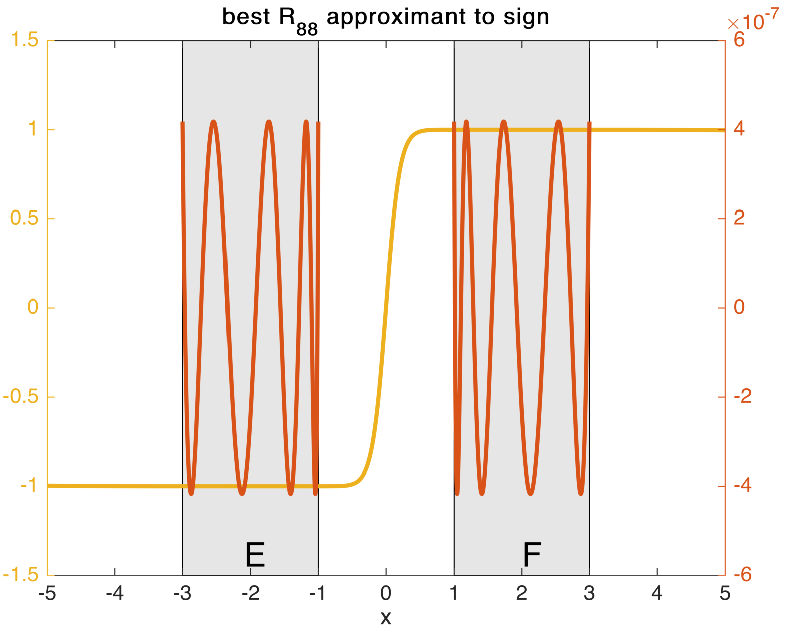
\includegraphics[width=\columnwidth]{Zolotarev-Solution.pdf}
	
	\onslide<2>{$\Rightarrow$ Zolotarev problem is then solved by solving for $Z_\ell(E,F)$.}
	\end{column}
	\end{columns}
	\end{frame}

	\begin{frame}[fragile]{The Zolotarev 3\textsuperscript{rd} Problem}
	\[
	\text{Solve for }Z_\ell(E,F)\text{ s.t. }\sup_{x \in [-b,1]\cup[1,b]} |R(x) - \operatorname{sgn}(x)| = \frac{\sqrt{Z_\ell(E,F)}}{1 + Z_\ell(E,F)}
	\]
	\begin{columns}
	\begin{column}{0.5\columnwidth}\definecolor{bg}{rgb}{0.95,0.95,0.95}
\begin{minted}[bgcolor=bg,fontsize=\footnotesize,breaklines]{matlab}
% Extrema for [-1,-1/b]\cup [1/b,1]:
K = ellipke(1-1/b^2);
[sn, cn, dn] = ellipj((0:k)*K/k, 1-1/b^2);
% Transplant to [-b,-1]\cup [1,b]:
extrema = b*dn;   
vals = 1-r(extrema);
c = mean( vals(1:2:end) );
e = eig( [ 2-4/c^2 1 ; 1 0 ] );
Zk = min(abs(e))
\end{minted}
	\end{column}
	\begin{column}{0.5\columnwidth}
	\centering
	
	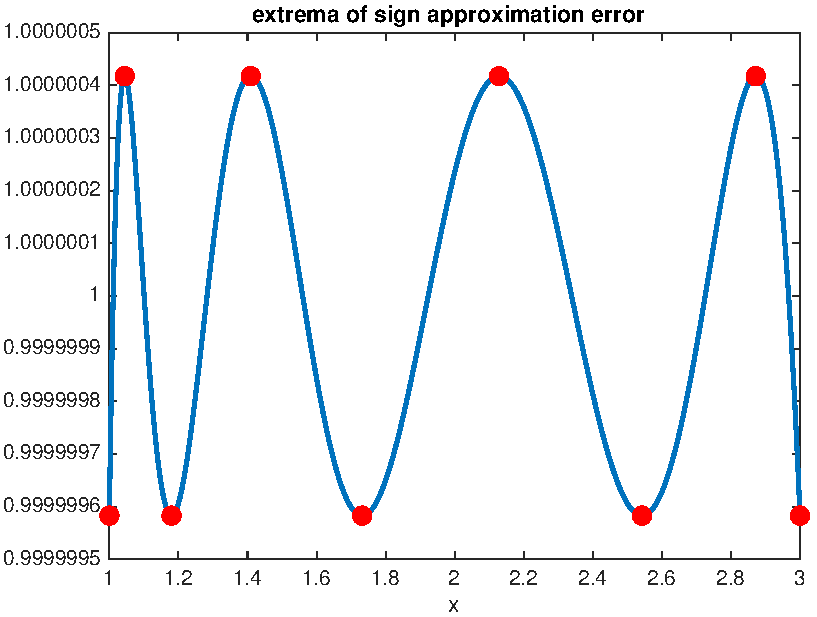
\includegraphics[width=0.8\columnwidth]{ExtremaZol.pdf}
	
	\end{column}
	\end{columns}

	From which we obtain \mintinline{matlab}{Zk = 4.3542e-14}.
	
	\end{frame}

	\begin{frame}[fragile]{The Zolotarev 3\textsuperscript{rd} Problem}
	To visualize the function realizing the extrema, one can use a Mobius transform to convert the best rational approximation to the $\operatorname{sgn}$ function that solves the 4\textsuperscript{th} problem $r(x)$ to the extremal rational function $R_{\ell,\ell}(x)$ solving the 3\textsuperscript{rd}:
	\begin{columns}
	\begin{column}{0.6\columnwidth}
	\[
	R_{\ell,\ell}(x) = \frac{\frac{1 + Z_\ell(E,F)}{ (1-Z_\ell(E,F))r(x) }}{\left( 1 - \frac{1+Z_\ell(E,F)}{1-Z_\ell(E,F)}r(x) \right)}
	\]	
	\begin{itemize}
		\item[\faCog]<2-> There are \textbf{other cases} for which one can solve the 3\textsuperscript{rd} problem, e.g., \emph{unsymmetrical intervals}, or \emph{rectangles} \parencite{MR1313712}.
		\item[\faHammer]<3-> If we are satisfied by the quasi-separability rank of the solution we can then attempt it!
	\end{itemize}
	\end{column}
	\begin{column}{0.4\columnwidth}
	\centering
	
	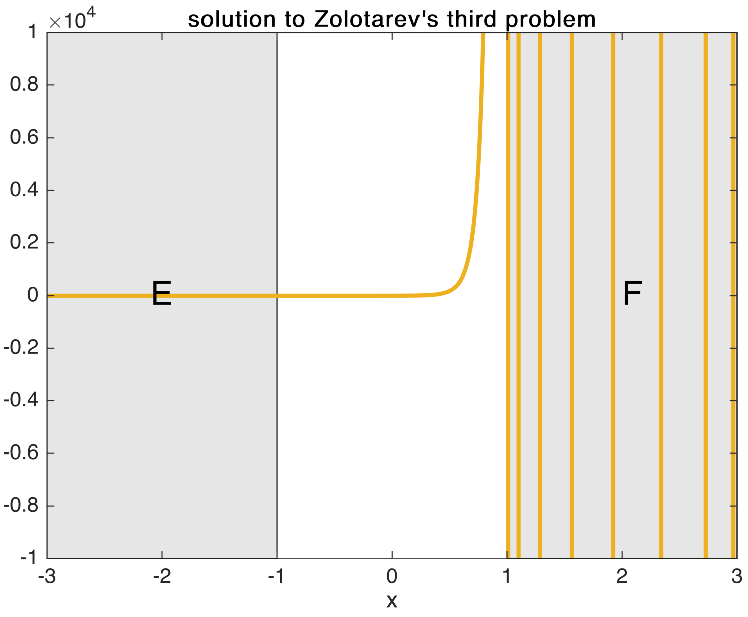
\includegraphics[width=\columnwidth]{ZoloFourSol.pdf}
	\end{column}
	\end{columns}
	\end{frame}

	\section{Conclusion and summary}
	
	\begin{frame}{Conclusion and summary}
	\definecolor{success}{HTML}{4a934a}
	\definecolor{todo}{HTML}{0099cc}
	
	\begin{itemize}
		\item[\textcolor{success}{\faCheckCircle}] We have reformulated several of our problems in terms of matrix equations,
		\item[\textcolor{success}{\faCheckCircle}] We have discussed projection methods for the solution of Sylvester equations,
		\item[\textcolor{success}{\faCheckCircle}] We have seen some limitations of the approach and shown a possible extension.
	\end{itemize}

	Next up
	\begin{itemize}
		\item[\textcolor{todo}{\faClipboardList}] More on rank-structured matrices and related solution strategies,
		\item[\textcolor{todo}{\faClipboardList}] All-at-once in time: using different methods to march in time than the standard ones,
		\item[\textcolor{todo}{\faClipboardList}] Still some other approaches with structured preconditioners.
	\end{itemize}
	
	\end{frame}
	
	\section*{Bibliography}
	{\unnumbered
		\begin{frame}[allowframebreaks,noframenumbering]{Bibliography}
			\small
			\printbibliography
			
		\end{frame}
	}
\end{document}